\documentclass[letterpaper]{article}

\usepackage{natbib,alifexi}
\usepackage{amsmath}
\usepackage[french]{babel}
\usepackage[utf8]{inputenc}
\usepackage{hyperref}
\usepackage[table,xcdraw]{xcolor}
\usepackage{amsfonts}
\usepackage{graphicx}
\usepackage{blkarray}
\usepackage{tikz}
\usetikzlibrary{automata, positioning}

\usepackage{fancyhdr}
\pagestyle{plain}

\newcommand{\colornode}[1][]{\node[state,
	    align=center,
	    text=gray!40!black,
	    draw=gray,
	    fill=gray!20!white,{#1}]}
\newcommand{\bigcolornode}[1][]{\node[state,
	    align=center,
	    text=gray!40!black,
	    draw=gray,
	    fill=gray!20!white,
	    text width=1.7cm,{#1}]}

\newcommand{\drawedge}{\draw[every loop, line width=0.4mm, fill=gray, draw=gray]}

% CASE evolution
\newcommand{\caseUp}[1][]{#1\textcolor[HTML]{008000}{$\mathbf{\uparrow}$}}
\newcommand{\caseStable}[1][]{#1\textcolor[HTML]{3779dd}{\textbf{-}}}
\newcommand{\caseDown}[1][]{#1\textcolor[HTML]{dd3737}{$\mathbf{\downarrow}$}}

\newcommand{\monopolyEditionAnni}{``Monopoly édition 70\up{ème} anniversaire''}

\title{Etude du Monopoly via les chaînes de Markov}
\author{Rémy Detobel\\
Mickael Randour\\
\mbox{}\\
Université Libre de Bruxelles, Bruxelles, Belgique \\
rdetobel@ulb.ac.be}


% =-=-=-=-=-=-=-=-= TODO GENERAL =-=-=-=-=-=-=-=-=
% - Pour l'économie, intéressant après 20 tours, 50, 100, ...


\begin{document}
\maketitle

\begin{abstract}
  Modélisation et étude du Monopoly à travers les chaînes de Markov.
  Les concepts principaux de ce modèle qu'est une chaîne de Markov
  seront présentés et expliqués.  Les différents choix permettant
  d'adapter le Monopoly afin qu'il puisse être modélisé comme une chaîne
  de Markov seront également justifiés.  Enfin, une description de
  l'application et des résultats récupérés par l'implémentation de cette
  modélisation sera également faite et permettra de déterminer les cases
  les plus fréquentées ainsi que les cases les plus rentables.
\end{abstract}

%%%%%%%%%%%%%% SECTION %%%%%%%%%%%%%%
\section{Introduction}
  Contrairement aux idées reçues, chaque case du Monopoly n'a pas la même
  probabilité d'être visitée.  Il est donc intéressant d'étudier quelles sont
  les cases les plus fréquentées mais également quelles seraient les cases
  les plus rentables.  Dans cette idée, il est possible de modéliser
  le Monopoly à travers les chaînes de Markov.  Mais avant cela, il est
  important de bien définir les chaînes de Markov ainsi que leurs propriétés.
  Les explications concernant ce modèle sont en grande partie basées
  sur le cours de M. \citet{COURS}.
  Pour pouvoir modéliser le Monopoly comme étant une chaîne de Markov,
  les règles du jeu doivent être clairement définies et des choix doivent
  être faits.  Ceux-ci seront donc expliqués et justifiés dans cet article.
  Les résultats trouvés suite à cette modélisation seront présentés afin
  de trouver, au final, les cases les plus visitées mais également les cases
  les plus rentables.
  % TODO ajouter des informations à l'intro (peut être plus conséquent)


%%%%%%%%%%%%%% SECTION %%%%%%%%%%%%%%
\section{Approche théorique}

  \subsection{Les chaînes de Markov}
    \label{def_chaine_markov}
    Une chaîne de Markov est une structure de données qui permet de modéliser l'évolution
    de l'état d'un système aléatoire.  Les chaînes de Markov sont basées sur le
    fait que l'état actuel du système dépend uniquement de l'état précédent.
    Cette propriété peut être appelée ``propriété de Markov''.  Une chaîne de
    Markov est donc composée d'états et de liens entre ces différents états caractérisés
    par une certaine probabilité de passer d'un état A à un état B.
    Cette probabilité sera décrite plus en détail dans le point \ref{probabilite}.
    Il est possible de représenter une chaîne de Markov de plusieurs manières différentes.
    Dans la littérature (comme par exemple dans le cours de M. \citet{COURS}), on utilisera
    plus souvent la notation matricielle, qui définit la chaîne de Markov $\mathcal{M}$
    telle que:
    $$\mathcal{M} = (S, \mathbf{P}, \iota_{init})$$
    Où $S$ représente l'ensemble de tous les états possibles, $\mathbf{P}$ une matrice $S \times S$
    où chaque élément est compris entre 0 et 1 et où cette valeur représente la probabilité
    de passer d'un état à un autre (respectivement, l'état correspondant à la ligne et à la colonne).
    On appellera cette matrice $\mathbf{P}$ la \textit{matrice de transition}.
    $\iota_{init}$ est une matrice colonne où chaque ligne représente un état et la valeur
    associée représente la probabilité de commencer par cet état.  On peut retrouver d'autres
    variables dans la littérature (comme $AP$ et $L$ par exemple pour associer des propositions
    atomiques aux états) mais celles-ci ne seront pas utiles dans cet article.
    Il est également possible de représenter une chaîne de Markov sous forme
    d'un graphe dirigé où chaque nœud représente un état et chaque arête est pondérée
    en fonction de la probabilité de passer d'un état à un autre.
    Notons également que les chaînes de Markov peuvent être utilisées
    dans un temps discret ou dans un temps continu.  Cependant, la modélisation
    du Monopoly n’inclura pas de temps continu et cet article traitera donc uniquement
    du temps discret.

  \subsection{Exemple de chaîne de Markov}
    \label{exemple}
    Afin d'illustrer les notions liées aux chaînes de Markov, cet article se
    basera sur un exemple représentant les différents états que peut avoir
    un avion.  On va donc ici considérer qu'un avion pourra avoir 6 états
    différents: \textit{en vol} (noté \textit{vol}), \textit{atterrissage}
    (noté \textit{att.}), \textit{décollage} (noté \textit{dec.}),
    \textit{au sol}, \textit{contrôle} (noté \textit{ctr.})
    et \textit{hors service} (noté \textit{h.s.}).
    On va considérer que lors de l'\textit{atterrissage}, il y a une chance sur
    3 pour qu'un voyant indique au pilote qu'un \textit{contrôle} est
    nécessaire. On remarque également qu'il y a une chance sur 10 que
    l'avion ne passe pas le \textit{contrôle} et soit considéré comme
    \textit{hors service}.  On considérera également que tous les avions commencent
    avec l'état \textit{au sol}.

    \subsubsection{Représentation matricielle}
      Comme vu au point \ref{def_chaine_markov}, il est possible de représenter une
      chaîne de Markov comme étant:
      $$\mathcal{M} = (S, \mathbf{P}, \iota_{init})$$
      Pour notre exemple on aura donc:
      $$S = \{vol, dec., att., sol, ctr., h.s.\} $$
      $$ \mathbf{P} =
	\begin{blockarray}{ccccccc}
	& vol & dec. & att. & sol & ctr. & h.s. \\
	  \begin{block}{c(cccccc)}
	    vol  & 0 & 0 & 1 & 0    & 0   & 0    \\
	    dec. & 1 & 0 & 0 & 0    & 0   & 0    \\
	    att. & 0 & 0 & 0 & 2/3  & 1/3 & 0    \\
	    sol  & 0 & 1 & 0 & 0    & 0   & 0    \\
	    ctr. & 0 & 0 & 0 & 9/10 & 0   & 1/10 \\
	    h.s. & 0 & 0 & 0 & 0    & 0   & 1    \\
	  \end{block}
	\end{blockarray}
      $$
      $$\iota_{init} =
	\begin{blockarray}{cc}
	  \begin{block}{( c ) c}
	    0 & vol \\
	    0 & dec.\\
	    0 & att.\\
	    1 & sol\\
	    0 & ctr.\\
	    0 & h.s.\\
	  \end{block}
	\end{blockarray}
      $$

    \subsubsection{Représentation graphique}
      Il est également possible de représenter cette chaîne de Markov comme
      étant un graphe dirigé (cfr point \ref{def_chaine_markov}):
      \begin{center}
	\begin{tikzpicture}
	  % Dessins des états
	  \colornode[text width=1.7cm] (vol) {En vol};

	  \colornode[below left=of vol] (att) {Atterrissage};
	  \bigcolornode[below right=of vol] (dec) {Décollage};

	  \bigcolornode[below right=of att] (sol) {Au sol};

	  \bigcolornode[below left=of sol] (ctr) {Contrôle};
	  \colornode[right=of ctr] (hs) {Hors service};

	  % Création des liens entre les états
	  \drawedge
	    (vol) edge[bend right, auto=right] node {1} (att)
	    (dec) edge[bend right, auto=right] node {1} (vol)
	    (sol) edge[bend right, auto=right] node {1} (dec)
	    (att) edge[bend right, auto=right] node {2/3} (sol)
	    (att) edge[bend right, auto=right] node {1/3} (ctr)
	    (ctr) edge[bend right, auto=left] node {9/10} (sol)
	    (ctr) edge[bend right, auto=right] node {1/10} (hs)
	    (hs) edge[loop right] node {1} (hs);
	  \draw [->, line width=0.4mm, fill=gray, draw=gray] (1.6,-5.4) -- (sol);
	\end{tikzpicture}
      \end{center}

  \subsection{Probabilité}
    \label{probabilite}
    La notion de probabilité peut se définir de plusieurs manières différentes
    et de nombreux ouvrages (comme par exemple celui de \citet{IP}) décrivent
    de manière très détaillée la notion de probabilité.  Dans ces ouvrages, on
    traite souvent des espaces de probabilité, qui demandent une approche très
    abstraite et rigoureuse.  Cependant dans cet article, l'approche
    fréquentielle inspirée des statistiques est suffisante.
    On définit donc la probabilité d'un événement aléatoire par la limite
    de la fréquence d’occurrence d'un événement pour un nombre d'expériences
    tendant vers l'infini.  De manière plus formelle, on peut décrire ce
    comportement comme $X$ étant une expérience aléatoire ayant
    $$\left\{X_i \mid i \in I\right\}$$
    pour résultats possibles, avec $I$ un ensemble d'indices (qui peuvent
    être finis, infinis dénombrables ou infinis non-dénombrables).  On définit
    la probabilité du résultat $X_i$ pour $i \in I$ par:
    $$\lim_{n \to \infty}\frac {X_i(n)}n,$$
    avec $X_i(n)$, le nombre d'occurrence du résultat $X_i$ lors de
    $n$ itérations de l'expérience $X$.  On note cette valeur
    $\mathbb P[X = X_i]$, si cette limite existe.
    Dans une chaîne de Markov on cherche à décrire l'évolution d'un état.
    L'évolution de cet état dépend d'événements aléatoires.  Il est donc tout
    a fait possible de définir une probabilité sur chacun des changements
    d'état possible dans la chaîne de Markov.

  \subsection{Simuler les changements d'état}
    Une chaîne de Markov permet donc d'estimer la probabilité de l'état
    futur d'un système uniquement en se basant sur l'état actuel du système.
    Dans cette idée, la matrice de transition $\mathbf{P}$ représente tous les
    déplacements d'une unité possible.  Si maintenant on veut connaître
    les états accessibles depuis notre état actuel après deux unités de temps,
    il suffit d'élever la matrice de transition au carré.  Si l'on reprend
    notre exemple, on aura donc:
    \begin{align*}
    \mathbf{P}^2 &=
      \begin{pmatrix}
	0 & 0 & 1 & 0    & 0   & 0    \\
	1 & 0 & 0 & 0    & 0   & 0    \\
	0 & 0 & 0 & 2/3  & 1/3 & 0    \\
	0 & 1 & 0 & 0    & 0   & 0    \\
	0 & 0 & 0 & 9/10 & 0   & 1/10 \\
	0 & 0 & 0 & 0    & 0   & 1    \\
      \end{pmatrix}^2\\
      &=
      \begin{pmatrix}
        0 & 0    & 0 & 2/3  & 1/3 & 0    \\
	0 & 0    & 1 & 0    & 0   & 0    \\
	0 & 2/3  & 0 & 3/10 & 0   & 1/30 \\
	1 & 0    & 0 & 0    & 0   & 0    \\
	0 & 9/10 & 0 & 0    & 0   & 1/10 \\
	0 & 0    & 0 & 0    & 0   & 1    \\
      \end{pmatrix}
    \end{align*}
    On remarque donc qu'après 2 déplacements depuis le premier état (première
    ligne), il sera possible d'atteindre le 4\up{ème} et 5\up{ème} état (avec
    respectivement une probabilité de $2/3$ et $1/3$).  Ce comportement est
    très simple à voir dans cet exemple, car l'état succédant à l'état 1 est
    obligatoirement le 3\up{ème} état.  Il est donc normal qu'après 2 tours,
    on retrouve les probabilités de déplacement du troisième état.

  \subsection{Propriété d'une chaîne de Markov}
    On peut remarquer que la somme de tous les éléments de chaque ligne de la
    matrice de transition fait $1$.  Ce phénomène peut également être vu
    sur la représentation graphique de la chaîne de Markov où la somme de chaque
    arête quittant un nœud (un état donc) vaut $1$.  Par exemple, si l'on se
    concentre sur l'état \textit{att.} (sur la représentation matricielle il s'agit donc
    de la 3\up{ème} ligne), on a bien: $2/3 + 1/3 + 0$ qui vaut bien $1$.  De manière
    plus formelle, cette caractéristique peut être notée telle que pour une matrice
    $\mathbf{P}$ (définie au point \ref{def_chaine_markov}) et pour tout état $s \in S$:
    $$\sum\limits_{s' \in S} \mathbf{P}(s, s') = 1$$
    Où $\mathbf{P}(s, s')$ représente la probabilité (présente dans la matrice de
    transition) de passer de l'état $s$ à l'état $s'$.  Cette caractéristique est
    toujours vraie par définition d'une chaîne de Markov mais également par définition
    d'une probabilité.
    En effet, la matrice $\mathbf{P}$ contient toutes les relations possibles entre
    tous les états du système ($S \times S$).  Une ligne représente donc toutes les
    relations possibles entre un état (définit par la ligne actuelle) et tous les autres
    états du système (les $S$ colonnes).  La probabilité de passer de l'état actuel
    à n'importe quel autre état du système est donc égale à $1$ (par définition d'une probabilité).
    Avec ce même raisonnement, il est logique de se rendre compte que la matrice
    de distribution initiale possède les mêmes caractéristiques:
    $$\sum\limits_{s \in S} \iota_{init}(s) = 1$$

  \subsection{Notation des chaînes des Markov}
    Certaines chaînes de Markov ont différentes structures et certains
    sous-ensembles d'états possèdent des caractéristiques particulières.
    Ces ensembles sont donc notés via différentes abréviations.  Ces différentes
    abréviations et concepts sont utilisés dans plusieurs articles scientifiques
    comme par exemple dans le livre de MM. \citet{ModelChecking} ou dans le cours
    M. \citet{COURS}.  Pour formaliser ces différents concepts, on définit
    une chaîne de Markov $\mathcal{M}(S, \mathbf{P}, \iota_{init})$
    (comme vu au point \ref{def_chaine_markov}) ainsi qu'un sous-ensemble $T$ de $S$.

    \subsubsection{Fortement connexe}
      Avant de définir la notion de fortement connexe, il faut définir la
      notion de \textit{chemin}.  Un tuple $(s_0,~\ldots, s_n) \in T^n$ est
      appelé \textit{chemin} si pour tout $i \in \{0,~\ldots, n-1\}$, 
      $\mathbf P(s_i, s_{i+1}) \neq 0$.
      Le sous-ensemble $T$ sera défini comme \textit{fortement connexe} si
      pour chaque paire d'états $(s, t)$ telle que $s, t \in T$, il existe un
      chemin $s_0, s_1, ..., s_n$ tel que $s_i \in T$ pour $0 \leq i \leq n$,
      $s_0 = s$ et $s_n = t$.\\
      Dans l'exemple présenté au point \ref{exemple}, une composante fortement
      connexe pourrait être: $\{vol, att., dec., sol\}$.

    \subsubsection{Composante fortement connexe}
      Une composante fortement connexe est abrégée \textit{SCC} (``Strongly
      Conntected Component'' en anglais).  Le sous-ensemble $T$ est une
      composante fortement connexe lorsque celui-ci est fortement connexe et
      que l'ajout d'un élément dans ce sous-ensemble violerait les propriétés
      définies par un ensemble fortement connexe.

    \subsubsection{BSCC}
      \label{bscc}
      \textit{BSCC} signifie ``Bottom Strongly Connected Component'' en anglais.
      Une \textit{BSCC} de $\mathcal{M}$ est une composante fortement connexe
      (SCC) $T$ tel qu'aucun état en dehors de $T$ n'est accessible.  De manière
      plus formelle, cela signifie que $\forall s \in T$:
      $$\sum\limits_{t \in T} \mathbf{P}(s, t) = 1$$
      L'exemple du point \ref{exemple} a pour seul BSCC: $\{h.s.\}$ (qui
      est donc uniquement composé d'un seul état).
      La propriété précédente nous apprend donc que lorsqu'un avion sera
      considéré comme \textit{hors service}, il n'y a aucun moyen de quitter
      cet état.  En effet, comme défini ci-dessus, tous les changements
      d'états pouvant être fait depuis un état présent dans un BSCC sont dirigés
      vers un état étant lui même présent dans ce BSCC.

  \subsection{Distribution stationnaire}
    \label{distribution_stationnaire}
    Comme vu au point \ref{bscc}, la probabilité de se retrouver dans un état
    présent dans un BSCC après un nombre fini ou infini dénombrable d'étapes est
    toujours de 1 (pour autant que l'on ait commencé dans un état lui-même présent
    dans ce BSCC).  Remarquons cependant que chaque état présent dans ce BSCC n'a
    pas la même probabilité d'être visitée.  En effet, certains états seront
    visités plus souvent que d'autres.
    On définit la distribution stationnaire comme étant un vecteur de probabilité
    $\mathbf{v}$ tel que:
    $$\mathbf{v}\mathbf{P} = \mathbf{v}$$
    et où pour chaque élément $\mathbf{v}_i \in \mathbf{v}, \mathbf{v}_i \in [0, 1]$.
    Par définition d'un BSCC, la somme des probabilités de chaque état doit valoir 1
    (car après un nombre fini ou infini dénombrable d'étapes, on sera toujours dans
    état présent dans ce même BSCC), on peut donc écrire:
    $$\sum\limits_{\mathbf{v}_i \in \mathbf{v}} \mathbf{v}_i = 1$$

    \subsubsection{Calcul de la distribution stationnaire}
      Nous allons définir le calcul de la distribution stationnaire à travers
      un exemple.  Malheureusement, il n'est pas possible de reprendre l'exemple
      présenté en point \ref{exemple} car le calcul de la distribution stationnaire
      de son BSCC est trivial (vu qu'il n'existe qu'un seul état dans ce BSCC) et vaut 1. 
      Nous allons donc légèrement modifier cet exemple en considérant maintenant
      que tous les avions \textit{hors service} seront tous réparés (avec une
      probabilité de 1 donc) et à nouveau mis dans l'état \textit{au sol}.
      Ce nouvel exemple sera noté $\mathcal{M}'$.
      La matrice de transition de $\mathcal{M}'$ sera donc:
      $$ \mathbf{P}' = 
	\begin{blockarray}{ccccccc}
	& vol & dec. & att. & sol & ctr. & h.s. \\
	  \begin{block}{c(cccccc)}
	    vol  & 0 & 0 & 1 & 0    & 0   & 0    \\
	    dec. & 1 & 0 & 0 & 0    & 0   & 0    \\
	    att. & 0 & 0 & 0 & 2/3  & 1/3 & 0    \\
	    sol  & 0 & 1 & 0 & 0    & 0   & 0    \\
	    ctr. & 0 & 0 & 0 & 9/10 & 0   & 1/10 \\
	    h.s. & 0 & 0 & 0 & 1    & 0   & 0    \\
	  \end{block}
	\end{blockarray}
      $$
      et sa représentation graphique:
      \begin{center}
	\begin{tikzpicture}
	  % Dessin des états
	  \colornode[text width=1.7cm] (vol) {En vol};

	  \colornode[below left=of vol] (att) {Atterrissage};
	  \bigcolornode[below right=of vol] (dec) {Décollage};

	  \bigcolornode[below right=of att] (sol) {Au sol};

	  \bigcolornode[below left=of sol] (ctr) {Contrôle};
	  \colornode[right=of ctr] (hs) {Hors service};

	  % Dessins des liens entre les états
	  \drawedge
	    (vol) edge[bend right, auto=right] node {1} (att)
	    (dec) edge[bend right, auto=right] node {1} (vol)
	    (sol) edge[bend right, auto=right] node {1} (dec)
	    (att) edge[bend right, auto=right] node {2/3} (sol)
	    (att) edge[bend right, auto=right] node {1/3} (ctr)
	    (ctr) edge[bend right, auto=left] node {9/10} (sol)
	    (ctr) edge[bend right, auto=right] node {1/10} (hs)
	    (hs) edge[bend right] node [left] {1} (sol);
	  \draw [->, line width=0.4mm, fill=gray, draw=gray] (1.6,-5.4) -- (sol);
	\end{tikzpicture}
      \end{center}
      Le BSCC de la matrice $\mathcal{M}'$ contiendra donc tous les états de cette
      chaîne de Markov.  Le calcul de la distribution stationnaire nous permet
      de connaître la probabilité de chaque état (présent dans ce BSCC) à être visité.
      La distribution stationnaire de la matrice $\mathcal{M}'$, sera donc définie
      par le vecteur $\mathbf{v}$ tel que:
      \begin{align*}
	\mathbf{v} . \mathbf{P}' &= \mathbf{v}\\
	\begin{blockarray}{(c)}
	  \mathbf{v}_{vol}\\
	  \mathbf{v}_{dec.}\\
	  \mathbf{v}_{att.}\\
	  \mathbf{v}_{sol}\\
	  \mathbf{v}_{ctr.}\\
	  \mathbf{v}_{h.s.}
	\end{blockarray}^T .
	\begin{blockarray}{(cccccc)}
	    0 & 0 & 1 & 0    & 0   & 0    \\
	    1 & 0 & 0 & 0    & 0   & 0    \\
	    0 & 0 & 0 & 2/3  & 1/3 & 0    \\
	    0 & 1 & 0 & 0    & 0   & 0    \\
	    0 & 0 & 0 & 9/10 & 0   & 1/10 \\
	    0 & 0 & 0 & 1    & 0   & 0    \\
	\end{blockarray}
	&=
	\begin{blockarray}{(c)}
	  \mathbf{v}_{vol}\\
	  \mathbf{v}_{dec.}\\
	  \mathbf{v}_{att.}\\
	  \mathbf{v}_{sol}\\
	  \mathbf{v}_{ctr.}\\
	  \mathbf{v}_{h.s.}
	\end{blockarray}^T
      \end{align*}
      et où:
      $$\mathbf{v}_{vol} + \mathbf{v}_{dec.} + \mathbf{v}_{att.} + \mathbf{v}_{sol} +
	\mathbf{v}_{ctr.} + \mathbf{v}_{h.s.} = 1$$
      Calculer une équation où les inconnues se trouvent de part et d'autre de l'égalité
      n'est pas une chose aisée, notons également que peu de solveurs acceptent les
      problèmes écrits de cette façon.  Il est donc possible de réécrire cette égalité
      de plusieurs manières différentes.  Le livre  ``Introduction to Probability''
      de \cite{IP} nous en présente quelques unes dans le chapitre 11.
      Dans cet article nous utiliserons une matrice identité $\mathbf{I}$ telle que:
      \begin{align*}
       \mathbf{v} . \mathbf{P}' &= \mathbf{v}\\
       \mathbf{v} . \mathbf{P}' &= \mathbf{v} . \mathbf{I}\\
       \mathbf{v} . \mathbf{P}' - \mathbf{v}. \mathbf{I} &= 0\\
       \mathbf{v} . (\mathbf{P}' - \mathbf{I}) &= 0
      \end{align*}
      On se retrouve donc avec un système d'équations plus ``classique'' (où chaque
      équation correspond à une constante):
      $$\begin{blockarray}{(c)}
	  \mathbf{v}_{vol}\\
	  \mathbf{v}_{dec.}\\
	  \mathbf{v}_{att.}\\
	  \mathbf{v}_{sol}\\
	  \mathbf{v}_{ctr.}\\
	  \mathbf{v}_{h.s.}
	\end{blockarray}^T .
	\begin{blockarray}{(cccccc)}
	    -1 & 0  & 1  & 0    & 0   & 0    \\
	    1  & -1 & 0  & 0    & 0   & 0    \\
	    0  & 0  & -1 & 2/3  & 1/3 & 0    \\
	    0  & 1  & 0  & -1   & 0   & 0    \\
	    0  & 0  & 0  & 9/10 & -1  & 1/10 \\
	    0  & 0  & 0  & 1    & 0   & -1    \\
	\end{blockarray}
	=
	\begin{blockarray}{(c)}
	  0\\
	  0\\
	  0\\
	  0\\
	  0\\
	  0
	\end{blockarray}^T$$
      Qui peut être décomposée en sous-équation:
      \begin{align*}
       \mathbf{v}_{vol} . -1 &+ \mathbf{v}_{dec.} . 1 &+ &\mathbf{v}_{att.} . 0 &+ ... &+ \mathbf{v}_{h.s} . 0 &= 0\\
       \mathbf{v}_{vol} . 0 &+ \mathbf{v}_{dec.} . -1 &+ &\mathbf{v}_{att.} . 0 &+ ... &+ \mathbf{v}_{h.s} . 0 &= 0\\
       & & ... & & & &= 0\\
       \mathbf{v}_{vol} . 0 &+ \mathbf{v}_{dec.} . 0 &+ &\mathbf{v}_{att.} . 0 &+ ... &+ \mathbf{v}_{h.s} . -1 &= 0\\
      \end{align*}
      Toutes les équations définissant la distribution stationnaire ont donc  la même forme:
      $$\mathbf{v}_{vol} + \mathbf{v}_{dec.} + \mathbf{v}_{att.} + \mathbf{v}_{sol} +
	\mathbf{v}_{ctr.} + \mathbf{v}_{h.s.} = 1$$
      La résolution de ce système d'équations nous permet donc de trouver la distribution
      stationnaire de notre chaîne de Markov $\mathcal{M}'$ qui vaut donc:
      \begin{align*}
       \mathbf{v} &= (\mathbf{v}_{vol}; \mathbf{v}_{dec.}; \mathbf{v}_{att.}; \mathbf{v}_{sol};
	  \mathbf{v}_{ctr.}; \mathbf{v}_{h.s.})\\
      \mathbf{v} &= (0,229; 0,229; 0,229; 0,229; 0,0763; 0,0076)
      \end{align*}


%%%%%%%%%%%%%% SECTION %%%%%%%%%%%%%%
\section{Modélisation}

  \subsection{Jeux de plateau}
    Plusieurs jeux de plateau peuvent être modélisés à travers une chaîne de Markov,
    comme par exemple le jeu de l'oie ou le Monopoly.  Dans ces jeux,
    la position du pion dépend uniquement de la case où il se trouvait précédemment.
    Comme vu dans le point \ref{def_chaine_markov}, les chaînes de Markov permettent
    de modéliser l'évolution de l'état d'un tel système.  La plupart du temps, dans
    la modélisation des jeux de plateau, on utilise la position du pion (sur le plateau)
    comme représentant l'état du système.  Cet état évolue donc avec le déplacement du
    pion.  La chaîne de Markov permet de prédire la probabilité que ce pion se retrouve
    sur une case donnée.  Les chaînes de Markov sont également basées sur le fait que
    l'évolution du système est dû à des événements aléatoires.  Il faut donc que le
    déplacement du pion soit lié à ces événements (aléatoires) comme par exemple le
    résultat d'un lancé de dés.

  \subsection{Modélisation}
    \label{modeliation_monopoly}
    Comme dit dans le point précédent, le Monopoly peut être modélisé par une chaîne de
    Markov.  On remarque également que tous les états composant cette chaîne de Markov
    appartiennent à un BSCC.  Plus concrètement, chaque case sera 
    numérotée et représentera un état de la chaîne de Markov.  L'état 2 de la chaîne
    de Markov représente le fait que le pion se trouve sur la case \textit{Caisse de
    communauté}.
    \begin{figure}[h]
      \centering
      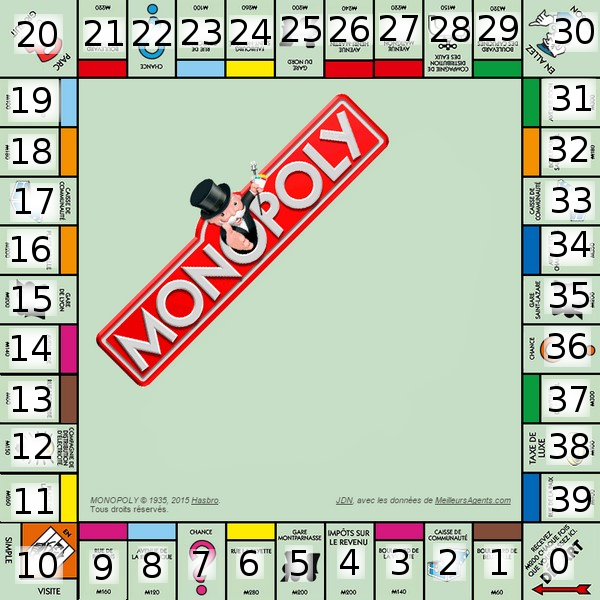
\includegraphics[scale=0.4]{./Images/Monopoly.png}
	\caption{Numérotation du Monopoly (basée sur une image venant du site
	\cite{IMG_Monopoly})}
    \end{figure}

    Chaque déplacement du pion (c'est-à-dire à chaque fois que l'on lance le dé) sera
    traduit par un changement d'état.
    Dans un premier temps, on modélise donc le Monopoly par 40 cases où chaque case est
    reliée aux $6 \times n-(n-1)$ cases suivantes à partir de la case $n-1$, où $n$ est le
    nombre de dé.  Dans le cas précis des règles du Monopoly (donc lorsque $n = 2$),
    chaque case pourra donc accéder à 11 autres cases.  En effet, le résultat le plus
    petit pouvant être produit par $n$ dés est de $n$ (tous les dé à 1).
    On devra donc éliminer toutes les $n-1$ cases juste après la case actuelle et le résultat
    le plus grand pouvant être produit par $n$ dés sera de $6 \times n$ (pour un dé à 6 faces).
    \begin{center}
      \begin{tikzpicture}
        \colornode[text width=1cm] at (0, 0) (c0) {Départ};
        \colornode[text width=0.7cm] at (1.5, 0) (c1) {Case 1};
        \colornode[text width=0.7cm] at (3, 0) (c2) {Case 2};
        \colornode[text width=1cm] at (5.5, 0) (cx) {...};
        \colornode[text width=0.7cm] at (7, 0) (c12) {Case 12};

        \drawedge
	  (c0) edge[bend left] node {} (c2)
	  (c0) edge[bend left] node {} (cx)
	  (c0) edge[bend left] node {} (c12)
	  (c1) edge[bend right] node {} (cx)
	  (c1) edge[bend right] node {} (c12);

      \end{tikzpicture}
    \end{center}
    Cependant, certaines cases ont un comportement particulier comme par exemple la
    case \textit{aller en prison}, la case \textit{Chance} ou encore la case
    \textit{Caisse de communauté}.  Les déplacements possibles à partir de ces cases
    ne sont pas les mêmes que pour les autres cases et seront donc étudiés dans les
    points suivants.

  \subsection{Répartition des dés}
    \label{repart_des}
    Lorsque l'on lance 2 dés, la somme des valeurs des dés n'a pas la même probabilité
    d'apparaître.  Il y a par exemple 3 manières différentes de former la valeur 4 (à
    savoir: $3+1$, $2+2$ et $1+3$) alors qu'il n'y a qu'une seule manière de former
    un 2 (à savoir: $1+1$).
    C'est ce que nous illustre la figure \ref{tableau_repartition_des}.  Sur celle-ci,
    on peut voir les cases jaunes aux extrémités qui représentent les valeurs que
    peuvent prendre chacun des dés.  Les cases bleues nous montrent la somme des valeurs
    de chaque dé.  Cette figure nous montre donc toutes les combinaisons possibles en
    lançant deux dés (et donc toutes les valeurs possibles).  On remarque par exemple
    qu'il y a 4 façons de faire un $5$ alors qu'il n'y a qu'une façon de faire un $2$.
    Cette image nous confirme également bien qu'il y a 36 combinaisons possibles
    lorsqu'on lance 2 dés.
    \begin{figure}[h]
      \centering
      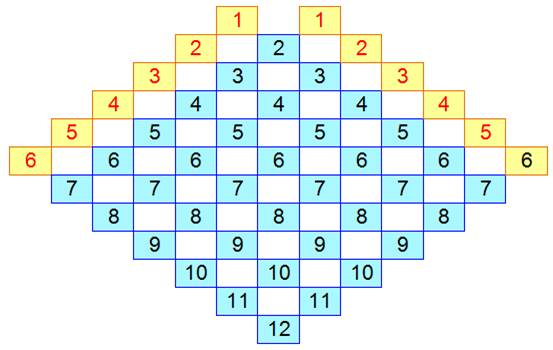
\includegraphics[scale=0.4]{./Images/RepartitionDes.jpg}
	\caption{Répartition des nombres formés avec 2 dés \citep{IMG_Des}}
      \label{tableau_repartition_des}
    \end{figure}

    \subsubsection{Calcul de la répartition des dés}
      L'explication intuitive du point \ref{repart_des} peut être généralisée.
      En effet, le Monopoly se joue avec deux dés.  Mais il pourrait être
      intéressant de voir le comportement du jeu avec un autre nombre de dés.
      On va donc s'intéresser à la répartition des valeurs obtenues lorsqu'on
      lance $n$ dés.  Le site \cite{FORMULE_Des} nous propose la formule
      suivante:
      $$\sum\limits_{k=0}^{(s-n)/6} (-1)^k \begin{pmatrix}n \\ k\end{pmatrix}
	\begin{pmatrix}s-6k-1 \\n-1\end{pmatrix}$$
      Où $n$ est le nombre de dés et $s$ le nombre que l'on désire former.
      Pour calculer la répartition totale, il suffit donc d'appliquer cette
      formule à tous les nombres pouvant être formés par $n$ dés.
      Cette équation est basée sur les fonctions génératrices permettant de
      trouver le nombre de combinaisons relatives à la somme de $n$ dés.
      Celle-ci peut donc être utilisée pour calculer la distribution
      des nombres pouvant être formés avec $n$ dés ayant n'importe quel
      nombre de face et n'importe quel valeur sur ces faces (tant que ce
      nombre soit naturel).
      Si l'on désire par exemple connaître la répartition d'un dé truqué
      ayant 3 faces $1$, 5 faces $2$ et une face $3$, on se basera sur le
      polynôme suivant: $3x + 5x^2 + x^3$.  Pour connaître la distribution
      des valeurs que l'on peut obtenir en lançant $n$ dés, il suffit de
      multiplier $n$ fois ce polynôme par lui-même.  Si on lance deux dés,
      on obtient donc:
      \begin{align*}
      &(3x + 5x^2 + x^3)^2\\
      &= (3x \times 3x) + (3x \times 5x^2) + (3x \times x^3) + (5x^2 \times 5x^2) + \\
      \tag*{$(5x^2 \times x^3) + (x^3 \times x^3)$}\\
      &= (9x^2) + (15x^3) + (3x^4) + (25x^4) + (5x^5) + (x^6)\\
      &= 1 x^6 + 5x^5 + 28x^4 + 15x^3 + 9x^2
      \end{align*}
      En faisant la somme des coefficients, on obtient le nombre d'arrangements
      possibles.  Dans le cas présent, on a donc $1 + 5 + 28 + 15 + 9$ c'est à
      dire $59$.  En regardant chaque monôme, on peut connaître la répartition
      de chaque valeur formée par le lancé de ces 2 dés truqués.  En effet,
      l'exposant nous donne le résultat formé et le coefficient permet de
      connaître sa probabilité.  Pour $9 x^2$ on peut donc déduire que la
      valeur $2$ aura une probabilité $9/59 = 0.15$ d'avoir lieu, ce même
      raisonnement peut être fait pour chacun des monômes.
      L'équation exprimée au début de ce point représente simplement le
      développement de ce polynôme.

  \subsection{Faire un double}
    Les règles du Monopoly stipulent que lorsque l'on fait 3 doubles
    consécutifs, on est directement envoyé en prison.
    \subsubsection{Modélisation}
      \label{modelisation_double}
      Pour modéliser ce comportement via une
      chaîne de Markov, il faut tripler le nombre d'états.  En effet, une case
      $i$ peut être visitée après avoir fait 0 double, 1 double ou 2 doubles.
      On peut donc représenter cela comme 3 plateaux de jeux parallèles comme
      montré sur la figure \ref{representation_double}.  A chaque fois que l'on
      fait un double, on se retrouve à un niveau ``plus bas'' (sur l'image).
      On a donc 3 niveaux: 0 où aucun double n'a encore été fait, 1 où le coup
      précédent était un double et le niveau 2 où les deux coups précédents
      étaient des doubles. Lorsque l'on fait un 3\up{ème} double, on se
      retrouve directement en prison.  Les flèches rouges sur la figure nous
      montrent les déplacements faits lorsque l'on obtient trois doubles
      consécutifs, à savoir dans le cas présent: $1+1$, $2+2$ et $6+6$.  Les
      flèches bleues nous montrent ce qui se passe lorsque l'on obtient un
      simple nombre (pas un double).  Elles sont toutes dirigées vers le
      plateau le plus haut sur l'image, c'est-à-dire celui où l'utilisateur
      n'a pas encore fait de double.
      \begin{figure}[h]
	\centering
	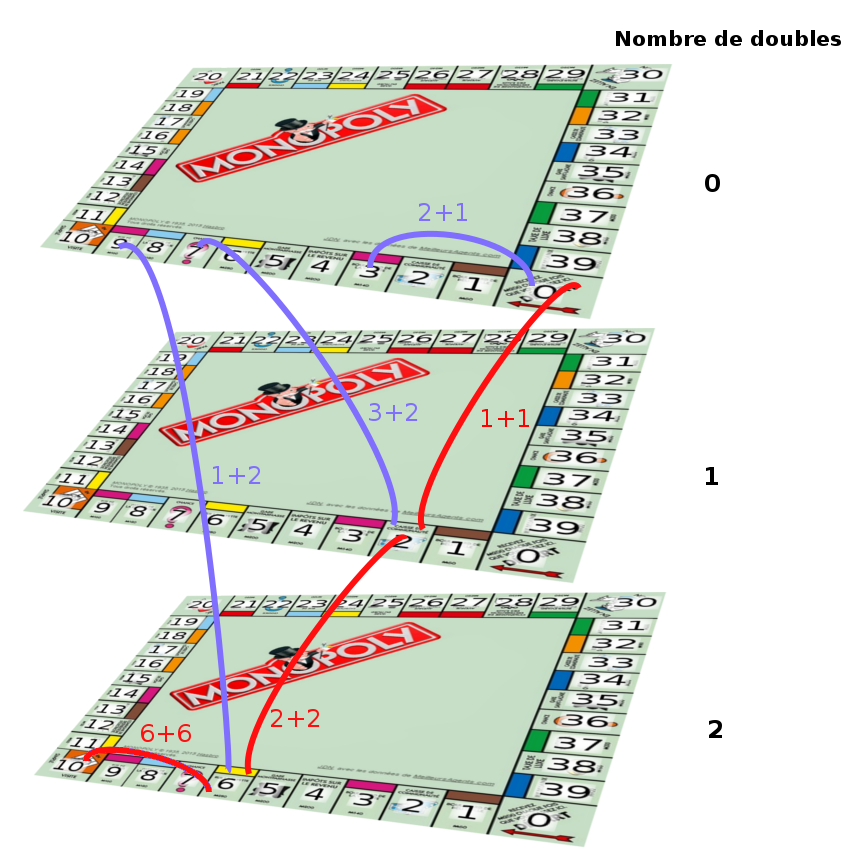
\includegraphics[scale=0.4]{./Images/MonopolyVertical_legende.png}
	  \caption{Déplacement en cas de double}
	  \label{representation_double}
      \end{figure}
      Dans cet article on considérera que le déplacement induit par une carte
      \textit{Chance} ou \textit{Caisse de communauté} fera redescendre le nombre
      de double à zéro.

    \subsubsection{Probabilité de faire un double}
      \label{prob_double}
      Comme vu dans le point \ref{repart_des}, il serait intéressant de
      pouvoir modéliser le Monopoly pour $n$ dés.  Il faut donc d'abord
      définir ce qu'est un \textit{double}.  Dans cet article, on va
      considérer que le joueur aura fait un double (au sens du Monopoly)
      si tous les nombres indiqués par les dés sont les mêmes. En d'autres
      mots, ce nombre est donc défini tel que $i \times n$ où $i$ est le nombre
      indiqué par tous les dés.  Par définition ce nombre est donc
      divisible par le nombre de dés.
      Il faut cependant bien tenir compte du fait qu'il y a plusieurs
      manières de former un même nombre.  Par exemple avec deux dés,
      il y a trois manières différentes de former le nombre $4$:
      $1+3$, $2+2$ et $3+1$.  Il y a donc 3 chance sur 36 de faire un
      $4$ mais seulement une chance sur 36 de faire un double.
      Pour une partie de Monopoly classique (où il y a donc seulement
      deux dés), il y a 6 chance sur 36 de faire un double, à savoir:
      $2$, $4$, $6$, $8$, $10$ et $12$.  Chaque double à une chance
      sur 36 d'apparaître.

  \subsection{Case \textit{prison}}
    \label{case_prison}
    Les règles du Monopoly stipulent que l'on peut sortir de prison de
    plusieurs manières différentes: soit via une carte chance, soit en
    payant, soit en faisant un double. Seul les deux dernières solutions
    seront utilisées dans cette modélisation. En effet, pour modéliser
    l'utilisation d'une carte permettant de sortir de prison, il faudrait,
    comme au point \ref{modelisation_double} dupliquer chaque case
    pour savoir si on est dans un état où l'on a une carte ou pas.
    Les règles indiquent également que l'on ne peut rester que 3 tours
    maximum avant d'être obligé de payer. Afin de représenter ces
    différents cas, la case prison sera triplée. On aura donc trois
    représentations de la case prison: au premier, second et troisième
    tour. La case \textit{aller en prison} sera donc considérée comme
    une case prison de niveau 0 et n'aura qu'une seule arête visant la
    case \textit{prison premier tour}. Comme vu au point \ref{prob_double},
    il y a une probabilité de $6/36$ de faire un double.  Dans les 5
    autres cas sur 6, on doit relancer le dés et on passera sur la case
    prison \textit{suivante}. Une fois arrivé sur la dernière case
    prison, on est obligé de payer.\\
    En résumé, il y a 7 déplacements possibles lorsque l'on sort de
    prison:
    \begin{itemize}
      \item faire un double (et avancer du résultat de ce double),
	ce qui correspond à 6 déplacements (à savoir: 2, 4, 6, 8, 10 et 12);
      \item payer et se retrouver sur la case \textit{prison visite
	uniquement}.
    \end{itemize}
    \textbf{Remarque:} les règles du Monopoly ne sont pas très claires
    quant au moment où l'on peut décider de payer pour sortir de prison.
    Soit le joueur a le droit de payer uniquement avant le premier tour
    passé en prison.  Soit le joueur peut reconsidérer cette offre à
    chaque tour passé en prison.  Dans cet article on considérera qu'il
    peut uniquement décider de payer pour sortir avant le premier tour.
    Il choisira cette option en fonction d'une probabilité définie (où
    1 correspondra au fait de payer à chaque fois pour sortir et 0
    d'attendre en espérant faire un double).

  \subsection{Case \textit{Aller en prison}}
    \label{aller_en_prison}
    La case \textit{Aller en prison} envoie directement le joueur vers
    la case prison.  Il est tout de même intéressant de connaître la
    probabilité de tomber sur cette case.  Elle a donc été modélise
    comme toutes les autres cases sauf qu'il y a une probabilité 1
    de se retrouver en prison le tour suivant.

  \subsection{Cases \textit{Chance}}
    Les cases \textit{Chance} font piocher une carte dans le paquet des
    cartes \textit{Chance}.  On suppose que chaque carte a la
    même probabilité d'être piochée. Ces cartes peuvent faire gagner de
    l'argent mais également déplacer les pions présents sur le plateau
    de jeu.  C'est évidemment ce second comportement qui sera étudié
    ici.  Le Monopoly comporte 16 cartes chances ayant la répartition
    suivante:
    \begin{itemize}
     \item 8 cartes faisant référence à des payements;
     \item une carte \textit{sortir de prison};
     \item 7 cartes faisant référence à un déplacement.
    \end{itemize}
    On peut donc en déduire que lorsqu'un joueur pioche une carte
    chance, il aura 7 chance sur 16 de devoir déplacer son pion.
    Ces déplacements sont les suivants:
    \begin{itemize}
     \item reculer de 3 cases;
     \item se rendre à la case départ;
     \item aller en prison;
     \item se rendre à la 11\up{ème} case (où 0 est le départ);
     \item se rendre à la 15\up{ème} case;
     \item se rendre à la 24\up{ème} case;
     \item se rendre à la 39\up{ème} case (dernière case avant l'arrivée).
    \end{itemize}
    Dans les 9 autres cas on lancera simplement les dés.  Les cases
    chances ont donc beaucoup d'arêtes.

  \subsection{Cases \textit{Caisse de communauté}}
    Comme les cases \textit{Chance}, les cases \textit{Caisse de
    communauté} font piocher une carte du même nom dans les mêmes
    condition que les cartes \textit{Chance}.  Les cartes
    \textit{Caisse de communauté} sont plus axées sur l'aspect
    financier du jeu. Cependant 3 cartes provoquent également des
    déplacements des pions:
    \begin{itemize}
     \item se rendre à la case départ;
     \item aller en prison;
     \item se rendre sur le première case.
    \end{itemize}
    La modélisation des cases \textit{Caisse de communauté} se fait de la
    même manière que les cases \textit{Chance}.

  \subsection{Probabilité de visiter une case}
    Comme introduit dans le point \ref{modeliation_monopoly}, le Monopoly
    peut être vu comme une chaîne de Markov et tous ses états appartiennent 
    à un BSCC.  On va donc utiliser la distribution stationnaire (présentée dans
    le point \ref{distribution_stationnaire}) afin de connaître la
    probabilité de visiter chaque case et en déduire quelle est la case la
    plus visitée.

  \subsubsection{Rentabilité}
    \label{rentabilite}
    Il y a plusieurs moyen de calculer la rentabilité d'une case.  Tout
    d'abord on peut simplement s'intéresser au nombre de fois que cette case
    devra être visitée pour permettre de la rentabiliser.  Cette information
    nous permettra juste de savoir quelle est la case qui a le plus haut revenu en
    fonction de son prix.\\
    Pour prendre en compte la probabilité qu'a un joueur de tomber sur cette
    case, il suffit de multiplier le revenu $r$ par la probabilité $p$ qu'elle soit
    visitée.  On a donc la formule suivante:
    $$r \times p = s$$
    Où $s$ est le revenu espéré par tour adverse.  C'est à dire qu'a chaque tour
    fait par un adversaire, on peut espérer récupérer la somme $s$ si l'on
    considère être dans un état stationnaire (et que la case est accessible
    pour l'adversaire).

\section{Résultats}
  Pour réduire la taille des tableaux et ne pas se baser sur les noms d'un seul
  Monopoly, les cases seront représentées par leur numéro.  Afin de tout de même 
  faciliter la lecture, les couleurs du Monopoly \monopolyEditionAnni
  seront appliquées.  Pour savoir plus précisément quel numéro
  correspond à quelle case, il faut consulter l'annexe \ref{liste_case}.  A noter
  également que toutes les valeurs chiffrées notamment utilisées dans l'annexe
  \ref{annexe:economie} viennent également du \monopolyEditionAnni.

  \subsection{Répartition des cases}

    \subsubsection{État stationnaire}
      Le but premier de cet article était de déterminer les cases ayant
      la plus grande probabilité d'être visitée.  Pour pouvoir répondre à
      cet objectif, on va se concentrer sur l'état stationnaire car il décrit
      au mieux le comportement des cases peu importe le nombre de tour considéré
      (pour autant que ce nombre soit assez important).  Il faut cependant
      prendre en compte plusieurs cas, car comme expliqué au point \ref{case_prison}, le
      joueur peut décider de payer directement pour sortir de prison ou bien
      essayer de faire un double.  On pourrait définir une probabilité par défaut
      avec lequel le joueur choisirait de payer ou pas.  Pour les résultats suivants,
      on a plutôt considéré le cas où il décidait de payer dès le début et un autre
      cas où le joueur décide de rester en prison et de ne payer que s'il a passé
      3 tours en prison.  Le tableau \ref{result_paye_pas} nous montre donc ce second
      cas de figure alors que le tableau \ref{result_paye} montre la répartition
      des cases si le joueur décide de directement payer pour sortir de prison.

      \begin{table}[h]
	\centering
	\begin{tabular}{|l|l||l|l|}
	  \hline
	  \multicolumn{1}{|c|}{{\textbf{N}}} & % Numero
	  \multicolumn{1}{c||}{\textbf{Probabilité}} & %
	  \multicolumn{1}{c|}{{\textbf{N}}} & % Numero
	  \multicolumn{1}{c|}{\textbf{Probabilité}} \\ \hline
	  \cellcolor[HTML]{000000} \textcolor{white}{41} & 3.474 \%  & \cellcolor[HTML]{FFD700} 30 & 2.32 \%  \\ \hline
	  \cellcolor[HTML]{000000} \textcolor{white}{42} & 2.895 \%  & \cellcolor[HTML]{483D8B} \textcolor{white}{40} & 2.305 \% \\ \hline
	  \cellcolor[HTML]{FF4500} 25 & 2.791 \%  & \cellcolor[HTML]{A0522D}  2 & 2.298 \% \\ \hline
	  \cellcolor[HTML]{FFFFFF}  1 & 2.711 \%  & \cellcolor[HTML]{2E8B57} 33 & 2.293 \% \\ \hline
	  \cellcolor[HTML]{FF8C00} 19 & 2.633 \%  & \cellcolor[HTML]{FF69B4} 15 & 2.273 \% \\ \hline
	  \cellcolor[HTML]{E6E6FA} 16 & 2.632 \%  & \cellcolor[HTML]{2E8B57} 35 & 2.171 \% \\ \hline
	  \cellcolor[HTML]{FFFFFF} 21 & 2.613 \%  & \cellcolor[HTML]{FFFFF0} 13 & 2.167 \% \\ \hline
	  \cellcolor[HTML]{FF8C00} 20 & 2.604 \%  & \cellcolor[HTML]{E6E6FA} 36 & 2.099 \% \\ \hline
	  \cellcolor[HTML]{FFC1C1} 23 & 2.59 \%   & \cellcolor[HTML]{8B1A1A}  \textcolor{white}{5} & 2.096 \% \\ \hline
	  \cellcolor[HTML]{FF8C00} 17 & 2.502 \%  & \cellcolor[HTML]{1E90FF}  9 & 2.079 \% \\ \hline
	  \cellcolor[HTML]{EEEED1} 18 & 2.449 \%  & \cellcolor[HTML]{FFC1C1}  8 & 2.078 \% \\ \hline
	  \cellcolor[HTML]{FF4500} 22 & 2.423 \%  & \cellcolor[HTML]{1E90FF}  7 & 2.05 \%  \\ \hline
	  \cellcolor[HTML]{000000} \textcolor{white}{43} & 2.413 \%  & \cellcolor[HTML]{1E90FF} 10 & 2.037 \% \\ \hline
	  \cellcolor[HTML]{FFD700} 27 & 2.394 \%  & \cellcolor[HTML]{FF69B4} 14 & 2.031 \% \\ \hline
	  \cellcolor[HTML]{E6E6FA} 26 & 2.389 \%  & \cellcolor[HTML]{000000} \textcolor{white}{11} & 2.002 \% \\ \hline
	  \cellcolor[HTML]{FF4500} 24 & 2.382 \%  & \cellcolor[HTML]{FFC1C1} 37 & 1.999 \% \\ \hline
	  \cellcolor[HTML]{FF69B4} 12 & 2.381 \%  & \cellcolor[HTML]{E6E6FA}  6 & 1.997 \% \\ \hline
	  \cellcolor[HTML]{FFD700} 28 & 2.379 \%  & \cellcolor[HTML]{A0522D}  4 & 1.944 \% \\ \hline
	  \cellcolor[HTML]{2E8B57} 32 & 2.36 \%   & \cellcolor[HTML]{EEEED1}  3 & 1.909 \% \\ \hline
	  \cellcolor[HTML]{EEEED1} 34 & 2.354 \%  & \cellcolor[HTML]{8B1A1A} 39 & 1.899 \% \\ \hline
	  \cellcolor[HTML]{FFFFF0} 29 & 2.346 \%  & \cellcolor[HTML]{483D8B} \textcolor{white}{38} & 1.893 \%  \\ \hline
	  \cellcolor[HTML]{BEBEBE} 31 & 2.345 \\ \cline{1-2}
	\end{tabular}
	\caption{Résultats si le joueur ne paye pas pour sortir de prison}
	\label{result_paye_pas}
      \end{table}

      \begin{table}[h]
	\centering
	\begin{tabular}{|l|l||l|l|}
	  \hline
	  \multicolumn{1}{|c|}{{\textbf{N}}} & % Numero
	  \multicolumn{1}{c||}{\textbf{Probabilité}} & %
	  \multicolumn{1}{c|}{{\textbf{N}}} & % Numero
	  \multicolumn{1}{c|}{\textbf{Probabilité}} \\ \hline
	  \cellcolor[HTML]{000000} \textcolor{white}{41} & 3.672 \%  & \cellcolor[HTML]{483D8B} \textcolor{white}{40} & 2.426 \% \\ \hline
	  \cellcolor[HTML]{FF4500} 25 & 2.956 \%  & \cellcolor[HTML]{2E8B57} 33 & 2.422 \% \\ \hline
	  \cellcolor[HTML]{E6E6FA} 16 & 2.889 \%  & \cellcolor[HTML]{FF69B4} 15 & 2.305 \% \\ \hline
	  \cellcolor[HTML]{FFFFFF}  1 & 2.866 \%  & \cellcolor[HTML]{2E8B57} 35 & 2.296 \% \\ \hline
	  \cellcolor[HTML]{FF8C00} 20 & 2.848 \%  & \cellcolor[HTML]{E6E6FA} 36 & 2.22 \%  \\ \hline
	  \cellcolor[HTML]{EEEED1} 18 & 2.76 \%   & \cellcolor[HTML]{8B1A1A}  \textcolor{white}{5} & 2.216 \% \\ \hline
	  \cellcolor[HTML]{FF8C00} 19 & 2.732 \%  & \cellcolor[HTML]{FF69B4} 14 & 2.209 \% \\ \hline
	  \cellcolor[HTML]{FFFFFF} 21 & 2.657 \%  & \cellcolor[HTML]{1E90FF}  9 & 2.198 \% \\ \hline
	  \cellcolor[HTML]{FF4500} 22 & 2.619 \%  & \cellcolor[HTML]{FFC1C1}  8 & 2.196 \% \\ \hline
	  \cellcolor[HTML]{FF8C00} 17 & 2.601 \%  & \cellcolor[HTML]{1E90FF}  7 & 2.167 \% \\ \hline
	  \cellcolor[HTML]{FFC1C1} 23 & 2.586 \%  & \cellcolor[HTML]{1E90FF} 10 & 2.153 \% \\ \hline
	  \cellcolor[HTML]{FFD700} 27 & 2.539 \%  & \cellcolor[HTML]{FFFFF0} 13 & 2.135 \% \\ \hline
	  \cellcolor[HTML]{E6E6FA} 26 & 2.539 \%  & \cellcolor[HTML]{000000} \textcolor{white}{11} & 2.117 \% \\ \hline
	  \cellcolor[HTML]{FF4500} 24 & 2.528 \%  & \cellcolor[HTML]{FFC1C1} 37 & 2.114 \% \\ \hline
	  \cellcolor[HTML]{FFD700} 28 & 2.517 \%  & \cellcolor[HTML]{E6E6FA}  6 & 2.111 \% \\ \hline
	  \cellcolor[HTML]{FF69B4} 12 & 2.508 \%  & \cellcolor[HTML]{A0522D}  4 & 2.054 \% \\ \hline
	  \cellcolor[HTML]{2E8B57} 32 & 2.492 \%  & \cellcolor[HTML]{EEEED1}  3 & 2.018 \% \\ \hline
	  \cellcolor[HTML]{EEEED1} 34 & 2.49 \%   & \cellcolor[HTML]{8B1A1A} 39 & 2.006 \% \\ \hline
	  \cellcolor[HTML]{FFFFF0} 29 & 2.478 \%  & \cellcolor[HTML]{483D8B} \textcolor{white}{38} & 2.0 \%   \\ \hline
	  \cellcolor[HTML]{BEBEBE} 31 & 2.473 \%  & \cellcolor[HTML]{000000} \textcolor{white}{42} & 0.0 \%   \\ \hline
	  \cellcolor[HTML]{FFD700} 30 & 2.447 \%  & \cellcolor[HTML]{000000} \textcolor{white}{43} & 0.0\%    \\ \hline
	  \cellcolor[HTML]{A0522D}  2 & 2.439 \\ \cline{1-2}
	\end{tabular}
	\caption{Résultats si le joueur paye directement pour
	  sortir de prison}
	\label{result_paye}
      \end{table}
      Outre le fait que dans le tableau \ref{result_paye} les cases \textit{prison} du
      2\up{ème} et 3\up{ème} tour sont à zéro, au profit de la 25\up{ème} case qui as
      encore plus de chance d'être visitée.  On peut remarque que ces deux tableaux
      mettent en évidence le fait que les cases prisons sont les plus visitées.
      Vient ensuite la case numéro 25 suivie des cases \textit{orange} (la couleur peut changer en
      fonction du Monopoly): 17, 19 et 20.  De manière générale, on remarque que se sont les cases
      ``au milieu'' du plateau (si l'on considère les cases 0 et 40 comme étant des extrémités) qui
      sont le plus visitées.  Cela peut s'expliquer par le fait que ce sont ces cases qui sont visitées
      par les joueurs sortant de prison.  Comme la case \textit{prison} a plus de chance
      d'être visitée dû aux nombreux moyens d'y arriver (voir le point \ref{case_prison}), il est
      normal que les cases accessibles en sortant de prison soient plus probablement visitées. Le fait
      que la case 25 soit la case achetable la plus visitée s'explique aussi par le fait qu'une
      cartes \textit{Chance} envoie directement le joueur sur ladite case.

    \subsubsection{Tour par tour}
      Le point précédent s'intéressait uniquement à la répartition des cases dans un état
      stationnaire.  Il peut cependant être intéressant de regarder la répartition des cases
      après un nombre fixé de tours.  On ne va cependant s'intéresser qu'aux résultats obtenus
      après 20 lancés.  En effet, avant cela il est possible qu'un joueur n'ait même pas encore
      fait un tour complet du plateau (vu que le nombre minimum pouvant être formé avec deux dés
      est de 2 et qu'il y a 40 cases).  Ces résultats sont tout de même disponibles sous forme de
      graphiques dans l'annexe \ref{annexe:graphe} (figure \ref{graph_result_paye_pas} et
      \ref{graph_result_paye}).  Les tableaux \ref{result_tour_paye_pas} et \ref{result_tour_paye}
      montrent donc la répartition des cases après 20, 40 et 60 tours.  Ces mêmes résultats
      sont également disponibles en annexe sous forme de graphique (également dans l'annexe
      \ref{annexe:graphe}, les figures \ref{graph_all_result_paye_pas} et \ref{graph_all_result_paye}).
      Ces tableaux mettent en relation une case avec la probabilité de tomber sur celle-ci en fonction du
      nombre de tours considéré.  Les cases sont ordonnées de la plus probable à la moins probable
      et un symbole permet d'indiquer si le résultat obtenu dans la colonne précédente (20 tours avant donc)
      plaçait la case dans une position inférieure, supérieure ou égale (respectivement \caseUp, \caseDown~
      et \caseStable) à la position actuelle de la case.

      \begin{table}
	\centering
	\begin{tabular}{|l|r||l|r||l|r|}
	  \hline
	  \multicolumn{1}{|c|}{{\textbf{N}}} & % Numero
	  \multicolumn{1}{p{1.5cm}||}{\centering \textbf{Probabilité \\ après 20 tours}} & %
	  \multicolumn{1}{c|}{{\textbf{N}}} & % Numero
	  \multicolumn{1}{p{1.5cm}||}{\centering \textbf{Probabilité \\ après 40 tours}} & %
	  \multicolumn{1}{c|}{{\textbf{N}}} & % Numero
	  \multicolumn{1}{p{1.5cm}|}{\centering \textbf{Probabilité \\ après 60 tours}} \\ \hline %
	  \cellcolor[HTML]{FF4500} 25 & 3.131 \% & \cellcolor[HTML]{000000} \textcolor{white}{41} & 3.517 \% \caseUp[\hfill] & \cellcolor[HTML]{000000} \textcolor{white}{41} & 3.47 \% \caseStable[\hfill] \\ \hline
	  \cellcolor[HTML]{FF8C00} 19 & 3.086 \% & \cellcolor[HTML]{000000} \textcolor{white}{42} & 2.926 \% \caseUp[\hfill] & \cellcolor[HTML]{000000} \textcolor{white}{42} & 2.893 \% \caseStable[\hfill] \\ \hline
	  \cellcolor[HTML]{FF8C00} 20 & 3.075 \% & \cellcolor[HTML]{FF4500} 25 & 2.762 \% \caseUp[\hfill] & \cellcolor[HTML]{FF4500} 25 & 2.793 \% \caseStable[\hfill] \\ \hline
	  \cellcolor[HTML]{FFFFFF} 21 & 3.068 \% & \cellcolor[HTML]{FFFFFF} 1  & 2.746 \% \caseUp[\hfill] & \cellcolor[HTML]{FFFFFF} 1 & 2.707 \% \caseStable[\hfill] \\ \hline
	  \cellcolor[HTML]{000000} \textcolor{white}{41} & 3.011 \% & \cellcolor[HTML]{E6E6FA} 16 & 2.6 \% \caseUp[\hfill] & \cellcolor[HTML]{FF8C00} 19 & 2.637 \% \caseUp[\hfill] \\ \hline
	  \cellcolor[HTML]{FFC1C1} 23 & 3.0 \% & \cellcolor[HTML]{FF8C00} 19 & 2.592 \% \caseDown[\hfill] & \cellcolor[HTML]{E6E6FA} 16 & 2.634 \% \caseDown[\hfill] \\ \hline
	  \cellcolor[HTML]{E6E6FA} 16 & 2.967 \% & \cellcolor[HTML]{FFFFFF} 21 & 2.572 \% \caseDown[\hfill] & \cellcolor[HTML]{FFFFFF} 21 & 2.616 \% \caseStable[\hfill] \\ \hline
	  \cellcolor[HTML]{EEEED1} 18 & 2.896 \% & \cellcolor[HTML]{FF8C00} 20 & 2.562 \% \caseDown[\hfill] & \cellcolor[HTML]{FF8C00} 20 & 2.607 \% \caseStable[\hfill] \\ \hline
	  \cellcolor[HTML]{FF8C00} 17 & 2.891 \% & \cellcolor[HTML]{FFC1C1} 23 & 2.554 \% \caseDown[\hfill] & \cellcolor[HTML]{FFC1C1} 23 & 2.593 \% \caseStable[\hfill] \\ \hline
	  \cellcolor[HTML]{FF4500} 22 & 2.87 \% & \cellcolor[HTML]{FF8C00} 17 & 2.467 \% \caseDown[\hfill] & \cellcolor[HTML]{FF8C00} 17 & 2.506 \% \caseStable[\hfill] \\ \hline
	  \cellcolor[HTML]{FF4500} 24 & 2.763 \% & \cellcolor[HTML]{EEEED1} 18 & 2.409 \% \caseDown[\hfill] & \cellcolor[HTML]{EEEED1} 18 & 2.453 \% \caseStable[\hfill] \\ \hline
	  \cellcolor[HTML]{E6E6FA} 26 & 2.688 \% & \cellcolor[HTML]{000000} \textcolor{white}{43} & 2.401 \% \caseUp[\hfill] & \cellcolor[HTML]{FF4500} 22 & 2.426 \% \caseUp[\hfill] \\ \hline
	  \cellcolor[HTML]{FFD700} 27 & 2.636 \% & \cellcolor[HTML]{FF4500} 22 & 2.384 \% \caseDown[\hfill] & \cellcolor[HTML]{000000} \textcolor{white}{43} & 2.414 \% \caseDown[\hfill] \\ \hline
	  \cellcolor[HTML]{FFD700} 28 & 2.559 \% & \cellcolor[HTML]{EEEED1} 34 & 2.377 \% \caseUp[\hfill] & \cellcolor[HTML]{FFD700} 27 & 2.395 \% \caseUp[\hfill] \\ \hline
	  \cellcolor[HTML]{FF69B4} 15 & 2.539 \% & \cellcolor[HTML]{FFD700} 27 & 2.374 \% \caseDown[\hfill] & \cellcolor[HTML]{E6E6FA} 26 & 2.391 \% \caseUp[\hfill] \\ \hline
	  \cellcolor[HTML]{000000} \textcolor{white}{42} & 2.537 \% & \cellcolor[HTML]{FF69B4} 12 & 2.373 \% \caseUp[\hfill] & \cellcolor[HTML]{FF4500} 24 & 2.385 \% \caseUp[\hfill] \\ \hline
	  \cellcolor[HTML]{000000} \textcolor{white}{43} & 2.512 \% & \cellcolor[HTML]{2E8B57} 32 & 2.371 \% \caseUp[\hfill] & \cellcolor[HTML]{FF69B4} 12 & 2.382 \% \caseDown[\hfill] \\ \hline
	  \cellcolor[HTML]{FFFFF0} 29 & 2.456 \% & \cellcolor[HTML]{FFD700} 28 & 2.364 \% \caseDown[\hfill] & \cellcolor[HTML]{FFD700} 28 & 2.38 \% \caseStable[\hfill] \\ \hline
	  \cellcolor[HTML]{FF69B4} 12 & 2.449 \% & \cellcolor[HTML]{E6E6FA} 26 & 2.364 \% \caseDown[\hfill] & \cellcolor[HTML]{2E8B57} 32 & 2.359 \% \caseDown[\hfill] \\ \hline
	  \cellcolor[HTML]{FFD700} 30 & 2.358 \% & \cellcolor[HTML]{BEBEBE} 31 & 2.35 \% \caseUp[\hfill] & \cellcolor[HTML]{EEEED1} 34 & 2.352 \% \caseDown[\hfill] \\ \hline
	  \cellcolor[HTML]{FFFFFF} 1 & 2.323 \% & \cellcolor[HTML]{FF4500} 24 & 2.349 \% \caseDown[\hfill] & \cellcolor[HTML]{FFFFF0} 29 & 2.346 \% \caseUp[\hfill] \\ \hline
	  \cellcolor[HTML]{BEBEBE} 31 & 2.311 \% & \cellcolor[HTML]{483D8B} \textcolor{white}{40} & 2.339 \% \caseUp[\hfill] & \cellcolor[HTML]{BEBEBE} 31 & 2.345 \% \caseDown[\hfill] \\ \hline
	  \cellcolor[HTML]{FFFFF0} 13 & 2.301 \% & \cellcolor[HTML]{FFFFF0} 29 & 2.338 \% \caseDown[\hfill] & \cellcolor[HTML]{FFD700} 30 & 2.32 \% \caseUp[\hfill] \\ \hline
	  \cellcolor[HTML]{2E8B57} 32 & 2.254 \% & \cellcolor[HTML]{A0522D} 2 & 2.332 \% \caseUp[\hfill] & \cellcolor[HTML]{483D8B} \textcolor{white}{40} & 2.302 \% \caseDown[\hfill] \\ \hline
	  \cellcolor[HTML]{FF69B4} 14 & 2.242 \% & \cellcolor[HTML]{FFD700} 30 & 2.318 \% \caseDown[\hfill] & \cellcolor[HTML]{A0522D} 2 & 2.295 \% \caseDown[\hfill] \\ \hline
	  \cellcolor[HTML]{2E8B57} 33 & 2.132 \% & \cellcolor[HTML]{2E8B57} 33 & 2.309 \% \caseStable[\hfill] & \cellcolor[HTML]{2E8B57} 33 & 2.291 \% \caseStable[\hfill] \\ \hline
	  \cellcolor[HTML]{EEEED1} 34 & 2.118 \% & \cellcolor[HTML]{FF69B4} 15 & 2.248 \% \caseDown[\hfill] & \cellcolor[HTML]{FF69B4} 15 & 2.276 \% \caseStable[\hfill] \\ \hline
	  \cellcolor[HTML]{000000} \textcolor{white}{11} & 2.013 \% & \cellcolor[HTML]{2E8B57} 35 & 2.196 \% \caseUp[\hfill] & \cellcolor[HTML]{2E8B57} 35 & 2.169 \% \caseStable[\hfill] \\ \hline
	  \cellcolor[HTML]{1E90FF} 10 & 1.989 \% & \cellcolor[HTML]{FFFFF0} 13 & 2.153 \% \caseDown[\hfill] & \cellcolor[HTML]{FFFFF0} 13 & 2.168 \% \caseStable[\hfill] \\ \hline
	  \cellcolor[HTML]{1E90FF} 9 & 1.977 \% & \cellcolor[HTML]{E6E6FA} 36 & 2.126 \% \caseUp[\hfill] & \cellcolor[HTML]{E6E6FA} 36 & 2.096 \% \caseStable[\hfill] \\ \hline
	  \cellcolor[HTML]{483D8B} \textcolor{white}{40} & 1.929 \% & \cellcolor[HTML]{8B1A1A} \textcolor{white}{5} & 2.12 \% \caseUp[\hfill] & \cellcolor[HTML]{8B1A1A} \textcolor{white}{5} & 2.094 \% \caseStable[\hfill] \\ \hline
	  \cellcolor[HTML]{FFC1C1} 8 & 1.922 \% & \cellcolor[HTML]{FFC1C1} 8 & 2.09 \% \caseStable[\hfill] & \cellcolor[HTML]{1E90FF} 9 & 2.078 \% \caseUp[\hfill] \\ \hline
	  \cellcolor[HTML]{A0522D} 2 & 1.919 \% & \cellcolor[HTML]{1E90FF} 9 & 2.085 \% \caseDown[\hfill] & \cellcolor[HTML]{FFC1C1} 8 & 2.077 \% \caseDown[\hfill] \\ \hline
	  \cellcolor[HTML]{2E8B57} 35 & 1.915 \% & \cellcolor[HTML]{1E90FF} 7 & 2.067 \% \caseUp[\hfill] & \cellcolor[HTML]{1E90FF} 7 & 2.049 \% \caseStable[\hfill] \\ \hline
	  \cellcolor[HTML]{1E90FF} 7 & 1.842 \% & \cellcolor[HTML]{1E90FF} 10 & 2.039 \% \caseDown[\hfill] & \cellcolor[HTML]{1E90FF} 10 & 2.037 \% \caseStable[\hfill] \\ \hline
	  \cellcolor[HTML]{8B1A1A} \textcolor{white}{5} & 1.819 \% & \cellcolor[HTML]{FFC1C1} 37 & 2.029 \% \caseUp[\hfill] & \cellcolor[HTML]{FF69B4} 14 & 2.033 \% \caseUp[\hfill] \\ \hline
	  \cellcolor[HTML]{E6E6FA} 36 & 1.809 \% & \cellcolor[HTML]{E6E6FA} 6 & 2.019 \% \caseUp[\hfill] & \cellcolor[HTML]{000000} \textcolor{white}{11} & 2.003 \% \caseUp[\hfill] \\ \hline
	  \cellcolor[HTML]{E6E6FA} 6 & 1.743 \% & \cellcolor[HTML]{FF69B4} 14 & 2.01 \% \caseDown[\hfill] & \cellcolor[HTML]{FFC1C1} 37 & 1.997 \% \caseDown[\hfill] \\ \hline
	  \cellcolor[HTML]{FFC1C1} 37 & 1.684 \% & \cellcolor[HTML]{000000} \textcolor{white}{11} & 1.999 \% \caseDown[\hfill] & \cellcolor[HTML]{E6E6FA} 6 & 1.996 \% \caseDown[\hfill] \\ \hline
	  \cellcolor[HTML]{A0522D} 4 & 1.614 \% & \cellcolor[HTML]{A0522D} 4 & 1.973 \% \caseStable[\hfill] & \cellcolor[HTML]{A0522D} 4 & 1.942 \% \caseStable[\hfill] \\ \hline
	  \cellcolor[HTML]{483D8B} \textcolor{white}{38} & 1.561 \% & \cellcolor[HTML]{EEEED1} 3 & 1.941 \% \caseUp[\hfill] & \cellcolor[HTML]{EEEED1} 3 & 1.906 \% \caseStable[\hfill] \\ \hline
	  \cellcolor[HTML]{EEEED1} 3 & 1.554 \% & \cellcolor[HTML]{8B1A1A} 39 & 1.932 \% \caseUp[\hfill] & \cellcolor[HTML]{8B1A1A} 39 & 1.896 \% \caseStable[\hfill] \\ \hline
	  \cellcolor[HTML]{8B1A1A} 39 & 1.54 \% & \cellcolor[HTML]{483D8B} \textcolor{white}{38} & 1.924 \% \caseDown[\hfill] & \cellcolor[HTML]{483D8B} \textcolor{white}{38} & 1.89 \% \caseStable[\hfill] \\ \hline
	\end{tabular}
	\caption{Résultats tour par tour si le joueur ne paye pas pour
	sortir de prison}
	\label{result_tour_paye_pas}
      \end{table}

      \begin{table}
	\centering
	\begin{tabular}{|l|r||l|r||l|r|}
	  \hline
	  \multicolumn{1}{|c|}{{\textbf{N}}} & % Numero
	  \multicolumn{1}{p{1.5cm}||}{\centering \textbf{Probabilité \\ après 20 tours}} & %
	  \multicolumn{1}{c|}{{\textbf{N}}} & % Numero
	  \multicolumn{1}{p{1.5cm}||}{\centering \textbf{Probabilité \\ après 40 tours}} & %
	  \multicolumn{1}{c|}{{\textbf{N}}} & % Numero
	  \multicolumn{1}{p{1.5cm}|}{\centering \textbf{Probabilité \\ après 60 tours}} \\ \hline %
	    \cellcolor[HTML]{000000} \textcolor{white}{41} & 3.485 \% & \cellcolor[HTML]{000000} \textcolor{white}{41} & 3.675 \% \caseStable[\hfill] & \cellcolor[HTML]{000000} \textcolor{white}{41} & 3.672 \% \caseStable[\hfill] \\ \hline
	    \cellcolor[HTML]{FF4500} 25 & 3.171 \% & \cellcolor[HTML]{FF4500} 25 & 2.948 \% \caseStable[\hfill] & \cellcolor[HTML]{FF4500} 25 & 2.956 \% \caseStable[\hfill] \\ \hline
	    \cellcolor[HTML]{FF8C00} 20 & 3.035 \% & \cellcolor[HTML]{E6E6FA} 16 & 2.89 \%  \caseUp[\hfill] & \cellcolor[HTML]{E6E6FA} 16 & 2.889 \% \caseStable[\hfill] \\ \hline
	    \cellcolor[HTML]{E6E6FA} 16 & 2.967 \% & \cellcolor[HTML]{FFFFFF}  1 & 2.872 \% \caseUp[\hfill] & \cellcolor[HTML]{FFFFFF} 1 & 2.866 \% \caseStable[\hfill] \\ \hline
	    \cellcolor[HTML]{FF8C00} 19 & 2.885 \% & \cellcolor[HTML]{FF8C00} 20 & 2.844 \% \caseDown[\hfill] & \cellcolor[HTML]{FF8C00} 20 & 2.848 \% \caseStable[\hfill] \\ \hline
	    \cellcolor[HTML]{EEEED1} 18 & 2.882 \% & \cellcolor[HTML]{EEEED1} 18 & 2.759 \% \caseStable[\hfill] & \cellcolor[HTML]{EEEED1} 18 & 2.76 \% \caseStable[\hfill] \\ \hline
	    \cellcolor[HTML]{FFFFFF} 21 & 2.856 \% & \cellcolor[HTML]{FF8C00} 19 & 2.73 \%  \caseDown[\hfill] & \cellcolor[HTML]{FF8C00} 19 & 2.732 \% \caseStable[\hfill] \\ \hline
	    \cellcolor[HTML]{FF4500} 22 & 2.832 \% & \cellcolor[HTML]{FFFFFF} 21 & 2.651 \% \caseDown[\hfill] & \cellcolor[HTML]{FFFFFF} 21 & 2.657 \% \caseStable[\hfill] \\ \hline
	    \cellcolor[HTML]{FFC1C1} 23 & 2.809 \% & \cellcolor[HTML]{FF4500} 22 & 2.613 \% \caseDown[\hfill] & \cellcolor[HTML]{FF4500} 22 & 2.619 \% \caseStable[\hfill] \\ \hline
	    \cellcolor[HTML]{FF4500} 24 & 2.755 \% & \cellcolor[HTML]{FF8C00} 17 & 2.601 \% \caseUp[\hfill] & \cellcolor[HTML]{FF8C00} 17 & 2.601 \% \caseStable[\hfill] \\ \hline
	    \cellcolor[HTML]{E6E6FA} 26 & 2.742 \% & \cellcolor[HTML]{FFC1C1} 23 & 2.579 \% \caseDown[\hfill] & \cellcolor[HTML]{FFC1C1} 23 & 2.587 \% \caseStable[\hfill] \\ \hline
	    \cellcolor[HTML]{FFD700} 27 & 2.725 \% & \cellcolor[HTML]{FFD700} 27 & 2.531 \% \caseStable[\hfill] & \cellcolor[HTML]{FFD700} 27 & 2.54 \% \caseStable[\hfill] \\ \hline
	    \cellcolor[HTML]{FF8C00} 17 & 2.703 \% & \cellcolor[HTML]{E6E6FA} 26 & 2.53 \%  \caseDown[\hfill] & \cellcolor[HTML]{E6E6FA} 26 & 2.539 \% \caseStable[\hfill] \\ \hline
	    \cellcolor[HTML]{FFD700} 28 & 2.681 \% & \cellcolor[HTML]{FF4500} 24 & 2.52 \%  \caseDown[\hfill] & \cellcolor[HTML]{FF4500} 24 & 2.529 \% \caseStable[\hfill] \\ \hline
	    \cellcolor[HTML]{FFFFFF}  1 & 2.667 \% & \cellcolor[HTML]{FF69B4} 12 & 2.513 \% \caseUp[\hfill] & \cellcolor[HTML]{FFD700} 28 & 2.517 \% \caseUp[\hfill] \\ \hline
	    \cellcolor[HTML]{FFFFF0} 29 & 2.616 \% & \cellcolor[HTML]{FFD700} 28 & 2.509 \% \caseDown[\hfill] & \cellcolor[HTML]{FF69B4} 12 & 2.508 \% \caseDown[\hfill] \\ \hline
	    \cellcolor[HTML]{FFD700} 30 & 2.556 \% & \cellcolor[HTML]{EEEED1} 34 & 2.487 \% \caseUp[\hfill] & \cellcolor[HTML]{2E8B57} 32 & 2.492 \% \caseUp[\hfill] \\ \hline
	    \cellcolor[HTML]{BEBEBE} 31 & 2.552 \% & \cellcolor[HTML]{2E8B57} 32 & 2.487 \% \caseUp[\hfill] & \cellcolor[HTML]{EEEED1} 34 & 2.49 \% \caseDown[\hfill] \\ \hline
	    \cellcolor[HTML]{2E8B57} 32 & 2.537 \% & \cellcolor[HTML]{FFFFF0} 29 & 2.47 \%  \caseDown[\hfill] & \cellcolor[HTML]{FFFFF0} 29 & 2.478 \% \caseStable[\hfill] \\ \hline
	    \cellcolor[HTML]{FF69B4} 12 & 2.479 \% & \cellcolor[HTML]{BEBEBE} 31 & 2.467 \% \caseDown[\hfill] & \cellcolor[HTML]{BEBEBE} 31 & 2.474 \% \caseStable[\hfill] \\ \hline
	    \cellcolor[HTML]{EEEED1} 34 & 2.458 \% & \cellcolor[HTML]{A0522D}  2 & 2.446 \% \caseUp[\hfill] & \cellcolor[HTML]{FFD700} 30 & 2.447 \% \caseUp[\hfill] \\ \hline
	    \cellcolor[HTML]{2E8B57} 33 & 2.436 \% & \cellcolor[HTML]{FFD700} 30 & 2.44 \%  \caseDown[\hfill] & \cellcolor[HTML]{A0522D} 2 & 2.439 \% \caseDown[\hfill] \\ \hline
	    \cellcolor[HTML]{FF69B4} 15 & 2.357 \% & \cellcolor[HTML]{483D8B} \textcolor{white}{40} & 2.43 \% \caseUp[\hfill] & \cellcolor[HTML]{483D8B} \textcolor{white}{40} & 2.426 \% \caseStable[\hfill] \\ \hline
	    \cellcolor[HTML]{483D8B} \textcolor{white}{40} & 2.248 \% & \cellcolor[HTML]{2E8B57} 33 & 2.418 \% \caseDown[\hfill] & \cellcolor[HTML]{2E8B57} 33 & 2.422 \% \caseStable[\hfill] \\ \hline
	    \cellcolor[HTML]{2E8B57} 35 & 2.247 \% & \cellcolor[HTML]{FF69B4} 15 & 2.306 \% \caseDown[\hfill] & \cellcolor[HTML]{FF69B4} 15 & 2.304 \% \caseStable[\hfill] \\ \hline
	    \cellcolor[HTML]{FF69B4} 14 & 2.235 \% & \cellcolor[HTML]{2E8B57} 35 & 2.294 \% \caseDown[\hfill] & \cellcolor[HTML]{2E8B57} 35 & 2.296 \% \caseStable[\hfill] \\ \hline
	    \cellcolor[HTML]{A0522D}  2 & 2.231 \% & \cellcolor[HTML]{8B1A1A} \textcolor{white}{5} & 2.223 \% \caseUp[\hfill] & \cellcolor[HTML]{E6E6FA} 36 & 2.22 \% \caseUp[\hfill] \\ \hline
	    \cellcolor[HTML]{E6E6FA} 36 & 2.142 \% & \cellcolor[HTML]{E6E6FA} 36 & 2.219 \% \caseStable[\hfill] & \cellcolor[HTML]{8B1A1A} \textcolor{white}{5} & 2.215 \% \caseDown[\hfill] \\ \hline
	    \cellcolor[HTML]{FFFFF0} 13 & 2.134 \% & \cellcolor[HTML]{FF69B4} 14 & 2.212 \% \caseDown[\hfill] & \cellcolor[HTML]{FF69B4} 14 & 2.209 \% \caseStable[\hfill] \\ \hline
	    \cellcolor[HTML]{1E90FF}  9 & 2.075 \% & \cellcolor[HTML]{1E90FF}  9 & 2.205 \% \caseStable[\hfill] & \cellcolor[HTML]{1E90FF} 9 & 2.197 \% \caseStable[\hfill] \\ \hline
	    \cellcolor[HTML]{1E90FF} 10 & 2.058 \% & \cellcolor[HTML]{FFC1C1}  8 & 2.204 \% \caseUp[\hfill] & \cellcolor[HTML]{FFC1C1} 8 & 2.196 \% \caseStable[\hfill] \\ \hline
	    \cellcolor[HTML]{000000} \textcolor{white}{11} & 2.053 \% & \cellcolor[HTML]{1E90FF}  7 & 2.175 \% \caseUp[\hfill] & \cellcolor[HTML]{1E90FF} 7 & 2.167 \% \caseStable[\hfill] \\ \hline
	    \cellcolor[HTML]{FFC1C1}  8 & 2.049 \% & \cellcolor[HTML]{1E90FF} 10 & 2.16 \% \caseDown[\hfill] & \cellcolor[HTML]{1E90FF} 10 & 2.153 \% \caseStable[\hfill] \\ \hline
	    \cellcolor[HTML]{8B1A1A}  \textcolor{white}{5} & 2.025 \% & \cellcolor[HTML]{FFFFF0} 13 & 2.139 \% \caseDown[\hfill] & \cellcolor[HTML]{FFFFF0} 13 & 2.135 \% \caseStable[\hfill] \\ \hline
	    \cellcolor[HTML]{FFC1C1} 37 & 2.008 \% & \cellcolor[HTML]{000000} \textcolor{white}{11} & 2.122 \% \caseDown[\hfill] & \cellcolor[HTML]{000000} \textcolor{white}{11} & 2.116 \% \caseStable[\hfill] \\ \hline
	    \cellcolor[HTML]{1E90FF}  7 & 1.998 \% & \cellcolor[HTML]{E6E6FA}  6 & 2.119 \% \caseUp[\hfill] & \cellcolor[HTML]{FFC1C1} 37 & 2.114 \% \caseUp[\hfill] \\ \hline
	    \cellcolor[HTML]{E6E6FA}  6 & 1.926 \% & \cellcolor[HTML]{FFC1C1} 37 & 2.114 \% \caseDown[\hfill] & \cellcolor[HTML]{E6E6FA} 6 & 2.11 \% \caseDown[\hfill] \\ \hline
	    \cellcolor[HTML]{483D8B} \textcolor{white}{38} & 1.871 \% & \cellcolor[HTML]{A0522D}  4 & 2.062 \% \caseUp[\hfill] & \cellcolor[HTML]{A0522D} 4 & 2.054 \% \caseStable[\hfill] \\ \hline
	    \cellcolor[HTML]{A0522D}  4 & 1.852 \% & \cellcolor[HTML]{EEEED1}  3 & 2.025 \% \caseUp[\hfill] & \cellcolor[HTML]{EEEED1} 3 & 2.017 \% \caseStable[\hfill] \\ \hline
	    \cellcolor[HTML]{8B1A1A} 39 & 1.85 \%  & \cellcolor[HTML]{8B1A1A} 39 & 2.01 \% \caseStable[\hfill] & \cellcolor[HTML]{8B1A1A} 39 & 2.006 \% \caseStable[\hfill] \\ \hline
	    \cellcolor[HTML]{EEEED1}  3 & 1.813 \% & \cellcolor[HTML]{483D8B} \textcolor{white}{38} & 2.002 \% \caseDown[\hfill] & \cellcolor[HTML]{483D8B} \textcolor{white}{38} & 2.0 \% \caseStable[\hfill] \\ \hline
	    \cellcolor[HTML]{000000} \textcolor{white}{42} & 0.0 \%   & \cellcolor[HTML]{000000} \textcolor{white}{42} & 0.0 \% \caseStable[\hfill] & \cellcolor[HTML]{000000} \textcolor{white}{42} & 0.0 \% \caseStable[\hfill] \\ \hline
	    \cellcolor[HTML]{000000} \textcolor{white}{43} & 0.0 \%   & \cellcolor[HTML]{000000} \textcolor{white}{43} & 0.0 \% \caseStable[\hfill] & \cellcolor[HTML]{000000} \textcolor{white}{43} & 0.0 \% \caseStable[\hfill] \\ \hline
	\end{tabular}
	\caption{Résultats tour par tour si le joueur paye pour
	sortir de prison}
	\label{result_tour_paye}
      \end{table}

      En comparant ces deux tableaux avec les tableaux du point précédent
      (à savoir \ref{result_paye_pas} et \ref{result_paye}), on constate
      qu'après 60 tours, l'ordre des cases est le même que si l'on était
      dans un état stationnaire.

    \subsubsection{Comparaison}
      Les résultats précédents peuvent être comparés à d'autres recherches déjà faites,
      comme par exemple la présentation de \cite{PP_MONOPOLY} où dans le 13\up{ème} slide
      on peut découvrir la liste des cases ainsi que la probabilité de tomber sur
      chacune d'entre elles lorsque le système est dans un état stationnaire.  Dans ce tableau, l'auteur
      ne distingue pas le nombre de tour passés en prison.  On remarque également
      que l'auteur a décidé de ne pas modéliser la case \textit{Aller en prison}
      contrairement au choix fait dans cet article en point \ref{aller_en_prison}.
      Dans cette même idée, les cases \textit{Chance} et \textit{Caisse de communauté}
      ont des probabilités plus faibles car l'auteur n'a compté aucune étape entre
      le fait que le pion tombe sur cette case et le fait que celui-ci doit être
      déplacé en fonction de l'action demandée par la carte.\\
      Bien que de nombreuses cases n'aient pas la même probabilité (pour les raisons
      expliquées ci-dessus), on peut tout de même constater que les trois premières cases
      du classement sont les mêmes: \textit{prison}, la 25\up{ème} case et la case départ.
      La case la moins chère du Monopoly, la 2\up{ème} case, se trouve au milieu du classement
      fait dans cet article alors que les résultats présents dans le document
      placent cette case tout en bas du classement.  Elle est pourtant visitée plus régulièrement
      suite à la possibilité de s'y rendre grâce à une carte \textit{Caisse de communauté}.
      De manière générale, on constate tout de même que les cases \textit{orange} et
      \textit{rouge} sont toujours au début du classement.
      % TODO comparaison avec l'autre document

  \subsection{Rentabilité}
    Comme vu dans le point \ref{rentabilite}, il y a plusieurs moyens
    de caractériser la rentabilité d'une case.  Un récapitulatif des cases
    ainsi que de leur coût, leur revenu ainsi que le ratio entre ces deux nombres
    est disponible dans l'annexe \ref{annexe:economie} (dans les tableaux
    \ref{table:rentabilite_paye} et \ref{table:rentabilite_paye_pas}).\\
    Ces chiffres ne tiennent pas compte de la répartition des cases décrite au
    point précédent.  Pour calculer la rentabilité d'une case, on peut
    se baser sur les calculs fait dans l'article écrit par \cite{MONOPOLY_ARTICLE} 
    et la présentation de \cite{PP_MONOPOLY} qui donne tous les deux des chiffres
    basé sur la couleur des cases.  En effet, ces deux articles se sont
    concentré sur un groupement de cases ayant un comportement similaire.
    La première étape est donc de regrouper les données utilisé dans 
    cet article de la même manière.  Le tableau \ref{result_cout_couleur} 
    nous montre donc le coût total d'un groupement de cases d'une certaines
    couleur en prenant en compte l'achat des appartements et des hotels.
    
    \begin{table}
      \centering
      \begin{tabular}{|c|r|}
	\hline
	\multicolumn{1}{|c|}{\textbf{Cases}} &
	\multicolumn{1}{c|}{\textbf{Coût total}} \\ \hline
	\cellcolor[HTML]{A0522D} 2, 4                      &  6200000 \$ \\ \hline
	\cellcolor[HTML]{1E90FF} 7, 9, 10                  & 10700000 \$ \\ \hline
	\cellcolor[HTML]{FF69B4} 12, 14, 15                & 19400000 \$ \\ \hline
	\cellcolor[HTML]{FF8C00} 17, 19, 20                & 20600000 \$ \\ \hline
	\cellcolor[HTML]{FF4500} 22, 24, 25                & 29300000 \$ \\ \hline
	\cellcolor[HTML]{FFD700} 27, 28, 30                & 30500000 \$ \\ \hline
	\cellcolor[HTML]{2E8B57} 32, 33, 35                & 39200000 \$ \\ \hline
	\cellcolor[HTML]{483D8B} \textcolor{white}{38, 40} & 27500000 \$ \\ \hline
      \end{tabular}
      \caption{Coût total d'achat des propriétés d'une même couleur avec des hotels}
      \label{table:result_cout_couleur}
    \end{table}
    
    On peut se rendre compte qu'a un facteur près, les valeurs 
    présente dans ce tableau corresponde à ceux présentes dans 
    le document de \cite{PP_MONOPOLY}.
    
    Les deux documents cité précédemment calculent le revenu
    espéré par groupe de propriété en fonction du nombre de
    tour adverse.  C'est ce qui a été fait dans le tableau
    \ref{result_revenu_couleur_paye} 
    
    Il nous reste donc encore
    à calculer le revenu moyen par tour adverse.  Pour cela on
    calcule d'abord le revenu moyen pour une couleur donnée.
    On additionne ensuite la somme des probabilités de chacune
    des cases relative à cette couleur.  Ensuite, on applique la
    formule expliqué en point \ref{rentabilite}.\\
    Le résultat de ce calcul est disponible dans le tableau 
    \ref{table:result_revenu_couleur_paye}.  On remarque bien
    qu'il s'agit des cases \textit{vertes} qui sont les plus 
    rentable et les cases 2 et 4 les moins rentables.
    
    \begin{table}
      \centering
      \begin{tabular}{|c|r|c|r|}
      \hline
      \multicolumn{1}{|c|}{\textbf{Cases}} &
      \multicolumn{1}{c|}{\textbf{Revenu moyen}} & 
      \multicolumn{1}{p{1.5cm}|}{\centering \textbf{Probabilité Total}} & 
      \multicolumn{1}{p{2cm}|}{\centering \textbf{Revenu moyen par tour adverse}} \\ \hline %
      \cellcolor[HTML]{A0522D} 2, 4                      &  3 500 000.00 \$ & 4.242 \% & 148 470.000 \$ \\ \hline
      \cellcolor[HTML]{1E90FF} 7, 9, 10                  &  5 666 666.66 \$ & 6.166 \% & 349 406.666 \$ \\ \hline
      \cellcolor[HTML]{FF69B4} 12, 14. 15                &  8 000 000.00 \$ & 6.685 \% & 534 800.000 \$ \\ \hline
      \cellcolor[HTML]{FF8C00} 17, 19, 20                &  9 666 666.66 \$ & 7.739 \% & 748 103.332 \$ \\ \hline
      \cellcolor[HTML]{FF4500} 22, 24, 25                & 10 666 666.66 \$ & 7.187 \% & 766 613.332 \$ \\ \hline
      \cellcolor[HTML]{FFD700} 27, 28, 30                & 11 666 666.66 \$ & 7.093 \% & 827 516.666 \$ \\ \hline
      \cellcolor[HTML]{2E8B57} 32, 33, 35                & 13 166 666.66 \$ & 6.824 \% & 898 493.332 \$ \\ \hline
      \cellcolor[HTML]{483D8B} \textcolor{white}{38, 40} & 17 500 000.00 \$ & 4.198 \% & 734 650.000 \$ \\ \hline
      \end{tabular}
      \caption{Revenu moyen pour un groupe de propriétés avec un hotel}
      \label{table:result_revenu_couleur_paye}
    \end{table}
    
    
\section{Conclusion}
  On constate qu'une chaîne de Markov est une bonne
  structure de données pour représenter un Monopoly.  Cette structure
  nous empêche cependant de calculer facilement le nombre de fois
  qu'un joueur visitera une case ou le fait qu'il ait une carte chance ou non.
  Plusieurs choix de modélisation n'ont pas eu beaucoup d'impact
  sur les résultats.  En effet, les cases les plus rentables restent les 
  cases \textit{orange} que l'on considère que le joueur paye
  directement pour sortir de prison ou non.  On constate également que
  la case la plus visitée reste bien la case prison suivie de la 25\up{ème}
  case du plateau.  On constate également que la probabilité de tomber sur
  une case devient très vite stable.  Après une cinquantaine de tours, la
  majorité des cases sont correctement classées.  On a également pu 
  constater que l'édition du Monopoly n'influençait en rien les résultats
  et de manière plus générale les conclusions que l'on pouvait en tirer.
  Bien que les valeurs soient différentes, elles sont toujours 
  proportionnelles.\\
  Les règles du Monopoly proposent une variante pour faire des parties
  rapides.  Cette variante propose de ne payer que la construction de 3 
  appartements pour faire un hotel.  Il serait intéressant de vérifier que
  cela ne modifie pas la rentabilité des cases. Cette variante propose
  également de terminer la partie lorsque deux joueurs sont en faillite.
  C'est alors le joueur ayant le plus d'argent qui remporte la partie.
  Cette modification impacte grandement le jeu car les joueurs devraient
  maintenant acheter des cases ayant une grande valeur marchande.  Enfin,
  cet article ne s'intéresse jamais aux valeurs hypothécaires des cases. 
  Il pourrait être intéressant de regarder quelle est la carte la plus 
  avantageuse à hypothéquer.
  
  
\footnotesize
\nocite{*}
\bibliographystyle{apalike}
\bibliography{Rapport}


\newpage
\appendix
  \pagenumbering{Roman}
  \onecolumn

  \section{Liste des cases}
    \label{liste_case}
    Les cases \textit{prison} sont numérotées à partir de 41 (la case \textit{prison} 2\up{ème} tour sera donc numérotée 42).\\
    \rotatebox{90}{
      \centering
      \begin{tabular}{|l|l|l|l|l|l|l|l|l|}
	  \hline
	  \multicolumn{1}{|c|}{} & % Numero
	  \multicolumn{2}{p{5cm}|}{\centering \textbf{Monopoly édition 70\up{ème} anniversaire}} &
	  \multicolumn{2}{p{4cm}|}{\centering \textbf{Monopoly Merveilles du monde}} &
	  \multicolumn{2}{p{4cm}|}{\centering \textbf{Monopoly Coupe du monde 2006}} &
	  \multicolumn{2}{p{4cm}|}{\centering \textbf{Monopoly Star Wars (ep2)}} \\ \hline
      1 & \cellcolor[HTML]{FFFFFF} & Départ & \cellcolor[HTML]{FFFFFF} & Départ & \cellcolor[HTML]{FFFFFF} & Départ & \cellcolor[HTML]{FFFFFF} & Départ \\ \hline
      2 & \cellcolor[HTML]{A0522D} & Wavre Rue du commerce & \cellcolor[HTML]{DA70D6} & Les Chutes du Niagara & \cellcolor[HTML]{DA70D6} & Australie & \cellcolor[HTML]{DA70D6} & Palais royal \\ \hline
      3 & \cellcolor[HTML]{EEEED1} & Caisse de Communauté & \cellcolor[HTML]{EEEED1} & Caisse de Communauté & \cellcolor[HTML]{EEEED1} & Caisse de Communauté & \cellcolor[HTML]{EEEED1} & Caisse de Communauté \\ \hline
      4 & \cellcolor[HTML]{A0522D} & Aalst Niewstraat & \cellcolor[HTML]{DA70D6} & L'Everest & \cellcolor[HTML]{DA70D6} & Suisse & \cellcolor[HTML]{DA70D6} & Retraite au bord du lac \\ \hline
      5 & \cellcolor[HTML]{8B1A1A} & Impôts sur le revenu & \cellcolor[HTML]{8B1A1A} & Assurance Voyage & \cellcolor[HTML]{8B1A1A} & Carton Rouge & \cellcolor[HTML]{8B1A1A} & Dégat d'astéroïde \\ \hline
      6 & \cellcolor[HTML]{E6E6FA} & Aéroport de Bruxelles Zaventem & \cellcolor[HTML]{E6E6FA} & Amsterdam Schiphol & \cellcolor[HTML]{E6E6FA} & Olympiastadium & \cellcolor[HTML]{E6E6FA} & Speeder de Zam Wesell \\ \hline
      7 & \cellcolor[HTML]{1E90FF} & Sint-truiden Luiderstraat & \cellcolor[HTML]{00BFFF} & La Grande Barrière de Corail & \cellcolor[HTML]{00BFFF} & Corée du sud & \cellcolor[HTML]{00BFFF} & Bureau de Palpatine \\ \hline
      8 & \cellcolor[HTML]{FFC1C1} & Chance & \cellcolor[HTML]{FFC1C1} & Chance & \cellcolor[HTML]{FFC1C1} & Chance & \cellcolor[HTML]{FFC1C1} & Chance \\ \hline
      9 & \cellcolor[HTML]{1E90FF} & Verviers place Verte & \cellcolor[HTML]{00BFFF} & Le Grand Canyon & \cellcolor[HTML]{00BFFF} & Tunisie & \cellcolor[HTML]{00BFFF} & Bibliothèque Jedi \\ \hline
      10 & \cellcolor[HTML]{1E90FF} & Mechelen Bruul & \cellcolor[HTML]{00BFFF} & Les chutes Angel & \cellcolor[HTML]{00BFFF} & Pologne & \cellcolor[HTML]{00BFFF} & Temple Jedi \\ \hline
      11 & \cellcolor[HTML]{000000} & Prison simple visite & \cellcolor[HTML]{FFFFFF} & Prison simple visite & \cellcolor[HTML]{FFFFFF} & Prison simple visite & \cellcolor[HTML]{FFFFFF} & Prison simple visite \\ \hline
      12 & \cellcolor[HTML]{FF69B4} & Arlon Grand'Rue & \cellcolor[HTML]{9932CC} & Le Christ Rédempteur & \cellcolor[HTML]{D02090} & Costa Rica & \cellcolor[HTML]{D02090} & Hangar de Speders \\ \hline
      13 & \cellcolor[HTML]{FFFFF0} & Telecoms & \cellcolor[HTML]{FFFFF0} & Bureau de Change & \cellcolor[HTML]{FFFFF0} & Distribution de boissons & \cellcolor[HTML]{FFFFF0} & Sabre laser \\ \hline
      14 & \cellcolor[HTML]{FF69B4} & Kortrijk Lange SteenStraat & \cellcolor[HTML]{9932CC} & La Tour Eiffel & \cellcolor[HTML]{D02090} & Croatie & \cellcolor[HTML]{D02090} & Nightclub Coruscant \\ \hline
      15 & \cellcolor[HTML]{FF69B4} & Mons Grand Rue & \cellcolor[HTML]{9932CC} & Le Colisée & \cellcolor[HTML]{D02090} & Iran & \cellcolor[HTML]{D02090} & Zone de Chargement \\ \hline
      16 & \cellcolor[HTML]{E6E6FA} & Aéroport de Charleroi & \cellcolor[HTML]{E6E6FA} & Paris Charles de Gaulle & \cellcolor[HTML]{E6E6FA} & Fritz-Walter-Stadion & \cellcolor[HTML]{E6E6FA} & Slave 1 \\ \hline
      17 & \cellcolor[HTML]{FF8C00} & Oostende Kapellestraat & \cellcolor[HTML]{FF8C00} & Les ruines de Stonehenge & \cellcolor[HTML]{FF8C00} & Alemagne & \cellcolor[HTML]{FF8C00} & Ferme de Cliegg Lars \\ \hline
      18 & \cellcolor[HTML]{EEEED1} & Caisse de Communauté & \cellcolor[HTML]{EEEED1} & Caisse de Communauté & \cellcolor[HTML]{EEEED1} & Caisse de Communauté & \cellcolor[HTML]{EEEED1} & Caisse de Communauté \\ \hline
      19 & \cellcolor[HTML]{FF8C00} & Leuven Bondgenotenlaan & \cellcolor[HTML]{FF8C00} & Le Taj Mahal & \cellcolor[HTML]{FF8C00} & Japon & \cellcolor[HTML]{FF8C00} & Plaine Désertiques \\ \hline
      20 & \cellcolor[HTML]{FF8C00} & Knokke Lippenslaan & \cellcolor[HTML]{FF8C00} & Les statues Moai & \cellcolor[HTML]{FF8C00} & Suède & \cellcolor[HTML]{FF8C00} & Camp de Jawa \\ \hline
      21 & \cellcolor[HTML]{FFFFFF} & Parking & \cellcolor[HTML]{FFFFFF} & Parking & \cellcolor[HTML]{FFFFFF} & Parking & \cellcolor[HTML]{FFFFFF} & Parking \\ \hline
      22 & \cellcolor[HTML]{FF4500} & Charleroi Rue de la Montagne & \cellcolor[HTML]{FF4500} & Machu Picchu & \cellcolor[HTML]{FF4500} & Italie & \cellcolor[HTML]{FF4500} & Kamino \\ \hline
      23 & \cellcolor[HTML]{FFC1C1} & Chance & \cellcolor[HTML]{FFC1C1} & Chance & \cellcolor[HTML]{FFC1C1} & Chance & \cellcolor[HTML]{FFC1C1} & Chance \\ \hline
      24 & \cellcolor[HTML]{FF4500} & Liège Rue de la Cathédrale & \cellcolor[HTML]{FF4500} & Le temple Angkor Wat & \cellcolor[HTML]{FF4500} & Portugal & \cellcolor[HTML]{FF4500} & Plateforme d'Atterrissage \\ \hline
      25 & \cellcolor[HTML]{FF4500} & Antwerpen Huidevetterstraat & \cellcolor[HTML]{FF4500} & Pétra & \cellcolor[HTML]{FF4500} & Angleterre & \cellcolor[HTML]{FF4500} & Entraînement de Clones \\ \hline
      26 & \cellcolor[HTML]{E6E6FA} & Aéroport de Liège & \cellcolor[HTML]{E6E6FA} & Rhein-Main Frankfurt & \cellcolor[HTML]{E6E6FA} & Zentralstadion & \cellcolor[HTML]{E6E6FA} & Starfighter Jedi \\ \hline
      27 & \cellcolor[HTML]{FFD700} & Hasselet Hoogstraat & \cellcolor[HTML]{FFD700} & La grande Muraille de Chine & \cellcolor[HTML]{FFD700} & USA & \cellcolor[HTML]{FFD700} & Cellule d'Obi-Wan \\ \hline
      28 & \cellcolor[HTML]{FFD700} & Brugge Steenstraat & \cellcolor[HTML]{FFD700} & Le phare d'Alexandrie & \cellcolor[HTML]{FFD700} & Mexique & \cellcolor[HTML]{FFD700} & Production de Droïde de combat \\ \hline
      29 & \cellcolor[HTML]{FFFFF0} & Internet & \cellcolor[HTML]{FFFFF0} & Agent de voyages & \cellcolor[HTML]{FFFFF0} & Compagnie d'éclairage & \cellcolor[HTML]{FFFFF0} & Telekinésie \\ \hline
      30 & \cellcolor[HTML]{FFD700} & Namur Rue de Fer & \cellcolor[HTML]{FFD700} & Le colosse de Rhodes & \cellcolor[HTML]{FFD700} & Espagne & \cellcolor[HTML]{FFD700} & Chaîne de Production droïde \\ \hline
      31 & \cellcolor[HTML]{BEBEBE} & Aller en prison & \cellcolor[HTML]{BEBEBE} & Aller en prison & \cellcolor[HTML]{BEBEBE} & Aller en prison & \cellcolor[HTML]{BEBEBE} & Aller en prison \\ \hline
      32 & \cellcolor[HTML]{2E8B57} & Bruxelles Av. Louise & \cellcolor[HTML]{2E8B57} & Le mausolée, Halicarnasse & \cellcolor[HTML]{2E8B57} & France & \cellcolor[HTML]{2E8B57} & Arène d'exécution \\ \hline
      33 & \cellcolor[HTML]{2E8B57} & Liège Pont d'Île & \cellcolor[HTML]{2E8B57} & La statue de Zeus, Olympie & \cellcolor[HTML]{2E8B57} & Argentine & \cellcolor[HTML]{2E8B57} & Loge pour VIP Géonosiens \\ \hline
      34 & \cellcolor[HTML]{EEEED1} & Caisse de Communauté & \cellcolor[HTML]{EEEED1} & Caisse de Communauté & \cellcolor[HTML]{EEEED1} & Caisse de Communauté & \cellcolor[HTML]{EEEED1} & Caisse de Communauté \\ \hline
      35 & \cellcolor[HTML]{2E8B57} & Gent Veldstraat & \cellcolor[HTML]{2E8B57} & Le temple d'Artémis à Ephèse & \cellcolor[HTML]{2E8B57} & Pays-Bas & \cellcolor[HTML]{2E8B57} & Suite secrète \\ \hline
      36 & \cellcolor[HTML]{E6E6FA} & Luchthaven Antwerpen & \cellcolor[HTML]{E6E6FA} & London Heathrow & \cellcolor[HTML]{E6E6FA} & Frankenstadion & \cellcolor[HTML]{E6E6FA} & Canonnière de République \\ \hline
      37 & \cellcolor[HTML]{FFC1C1} & Chance & \cellcolor[HTML]{FFC1C1} & Chance & \cellcolor[HTML]{FFC1C1} & Chance & \cellcolor[HTML]{FFC1C1} & Chance \\ \hline
      38 & \cellcolor[HTML]{483D8B} & Antwerpen Meir & \cellcolor[HTML]{483D8B} & Jardins suspendus de Babylone & \cellcolor[HTML]{483D8B} & République Tchèque & \cellcolor[HTML]{483D8B} & Armée de Droïde de combat \\ \hline
      39 & \cellcolor[HTML]{8B1A1A} & Taxe de Luxe & \cellcolor[HTML]{8B1A1A} & Taxe de Luxe & \cellcolor[HTML]{8B1A1A} & Carton jaune & \cellcolor[HTML]{8B1A1A} & Homme des sables \\ \hline
      40 & \cellcolor[HTML]{483D8B} & Bruxelles Rue Neuve & \cellcolor[HTML]{483D8B} & La grande Pyramide de Gizeh &\cellcolor[HTML]{483D8B} & Brésil &\cellcolor[HTML]{483D8B} & Armée Clone\\ \hline
      \end{tabular}
    }

    \newpage

    \section{Graphique}
      \label{annexe:graphe}
      \subsection{Répartition des cases}
	\begin{center}
	  \begin{figure}[bp!]
	    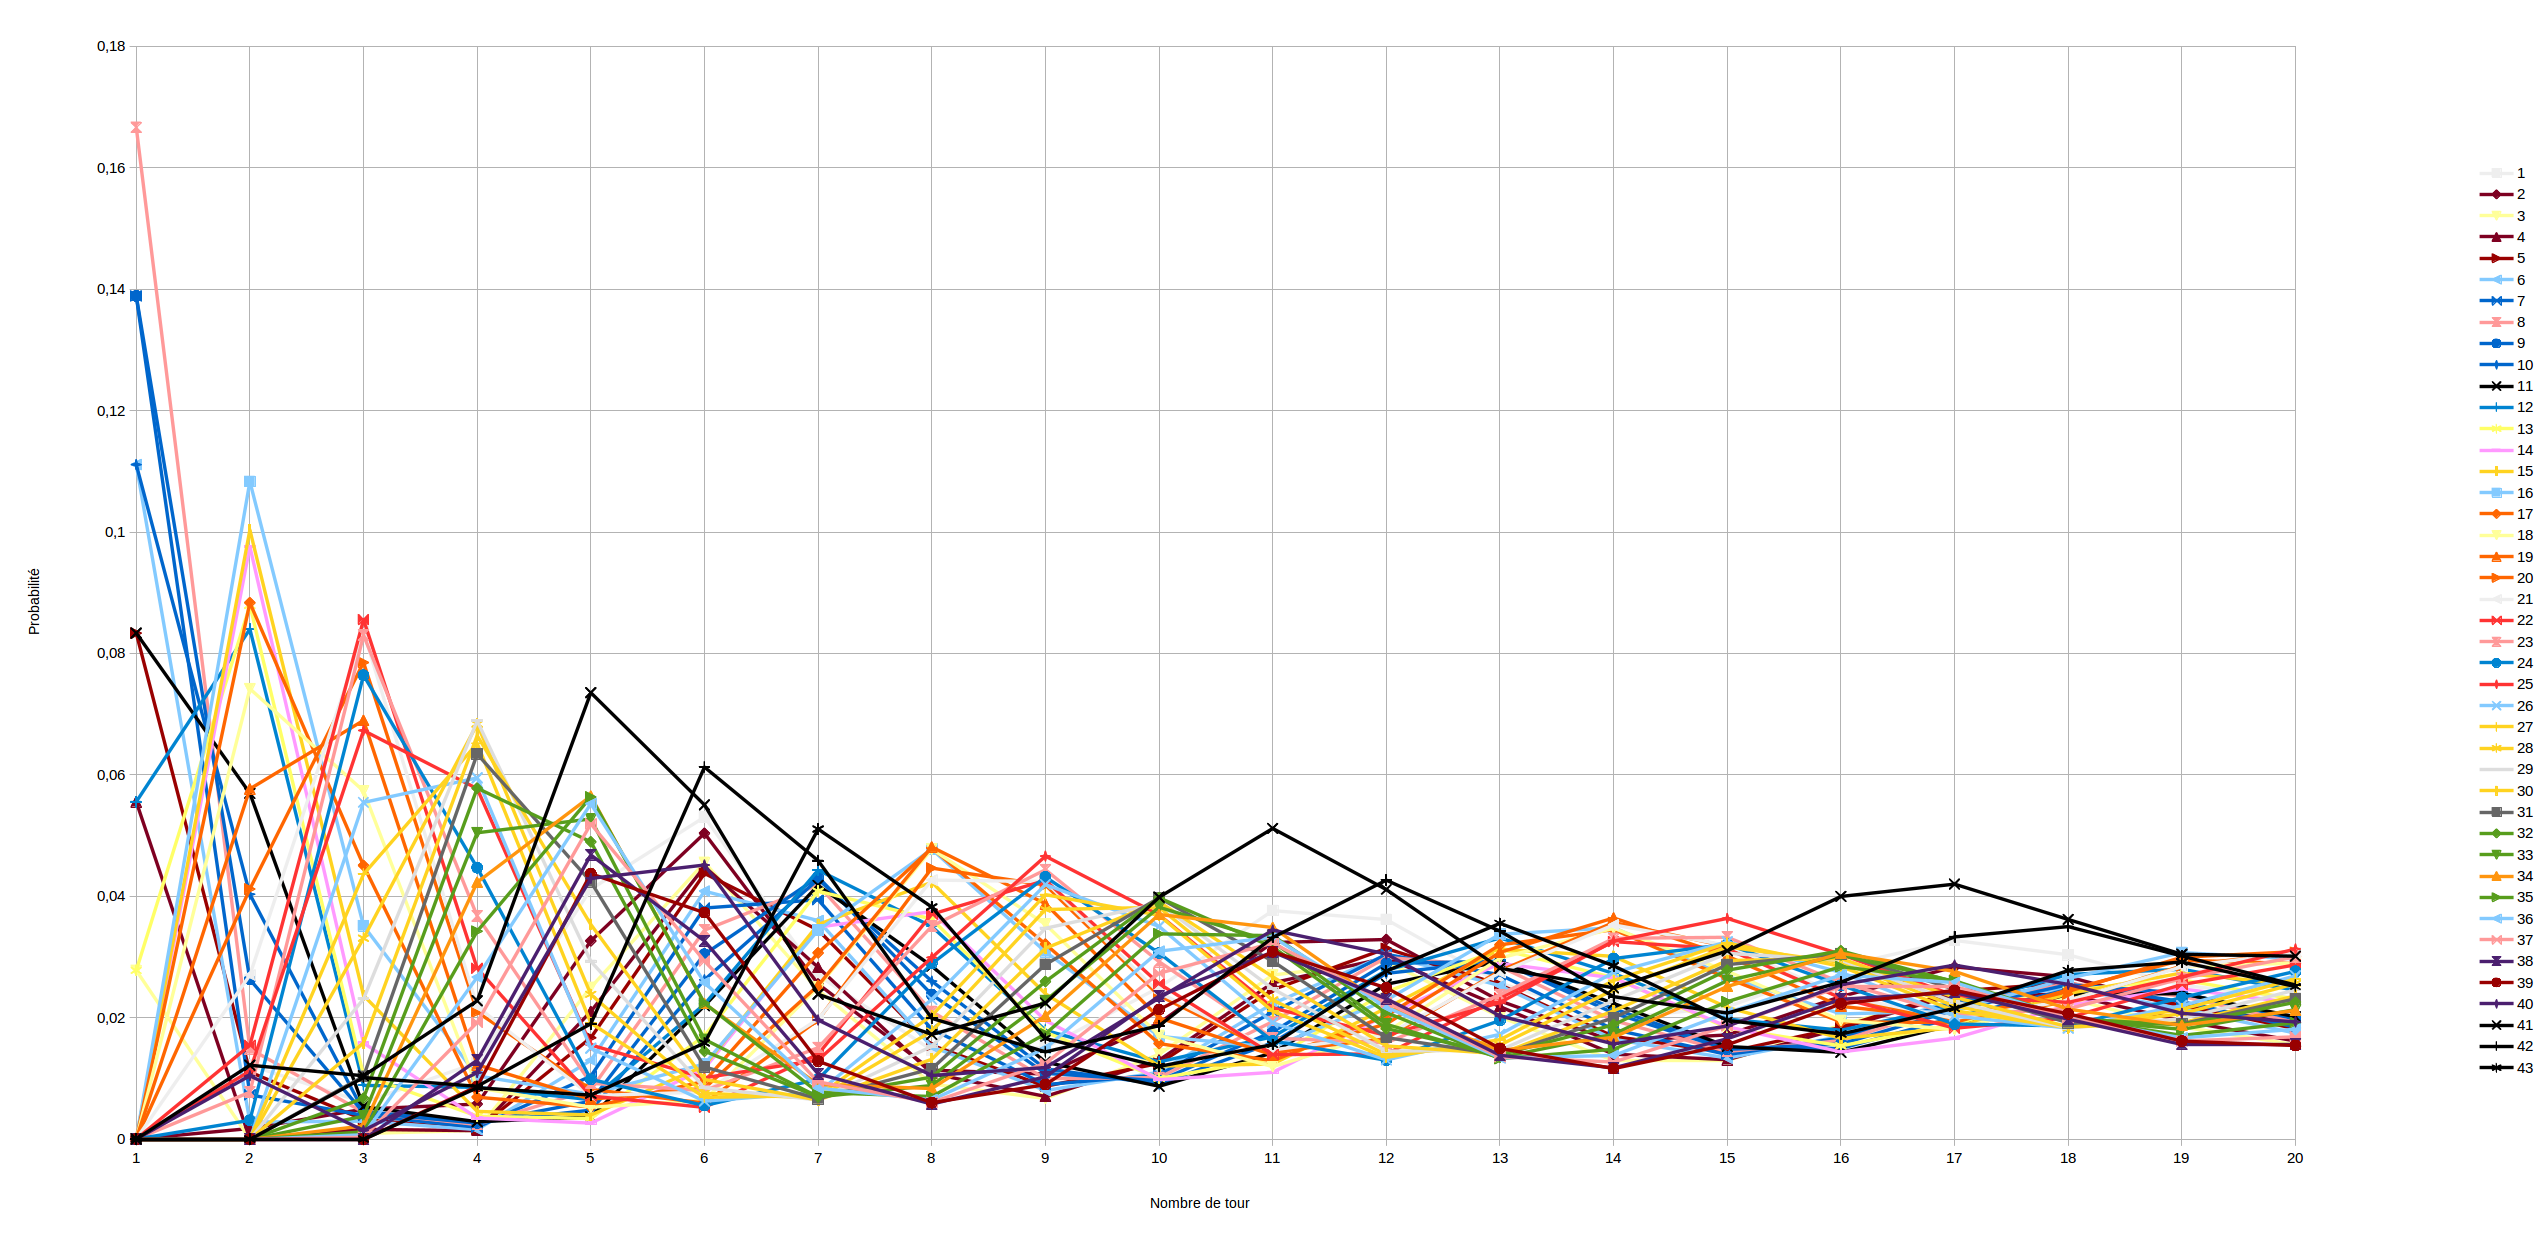
\includegraphics[scale=0.26]{./Images/GraphRepPayePasLeq20.png}
	    \caption{\label{graph_result_paye_pas} Répartition des cases entre 1 et 20 tours lorsque le joueur ne paye pas pour sortir de prison}
	  \end{figure}

	  \begin{figure}[bp!]
	    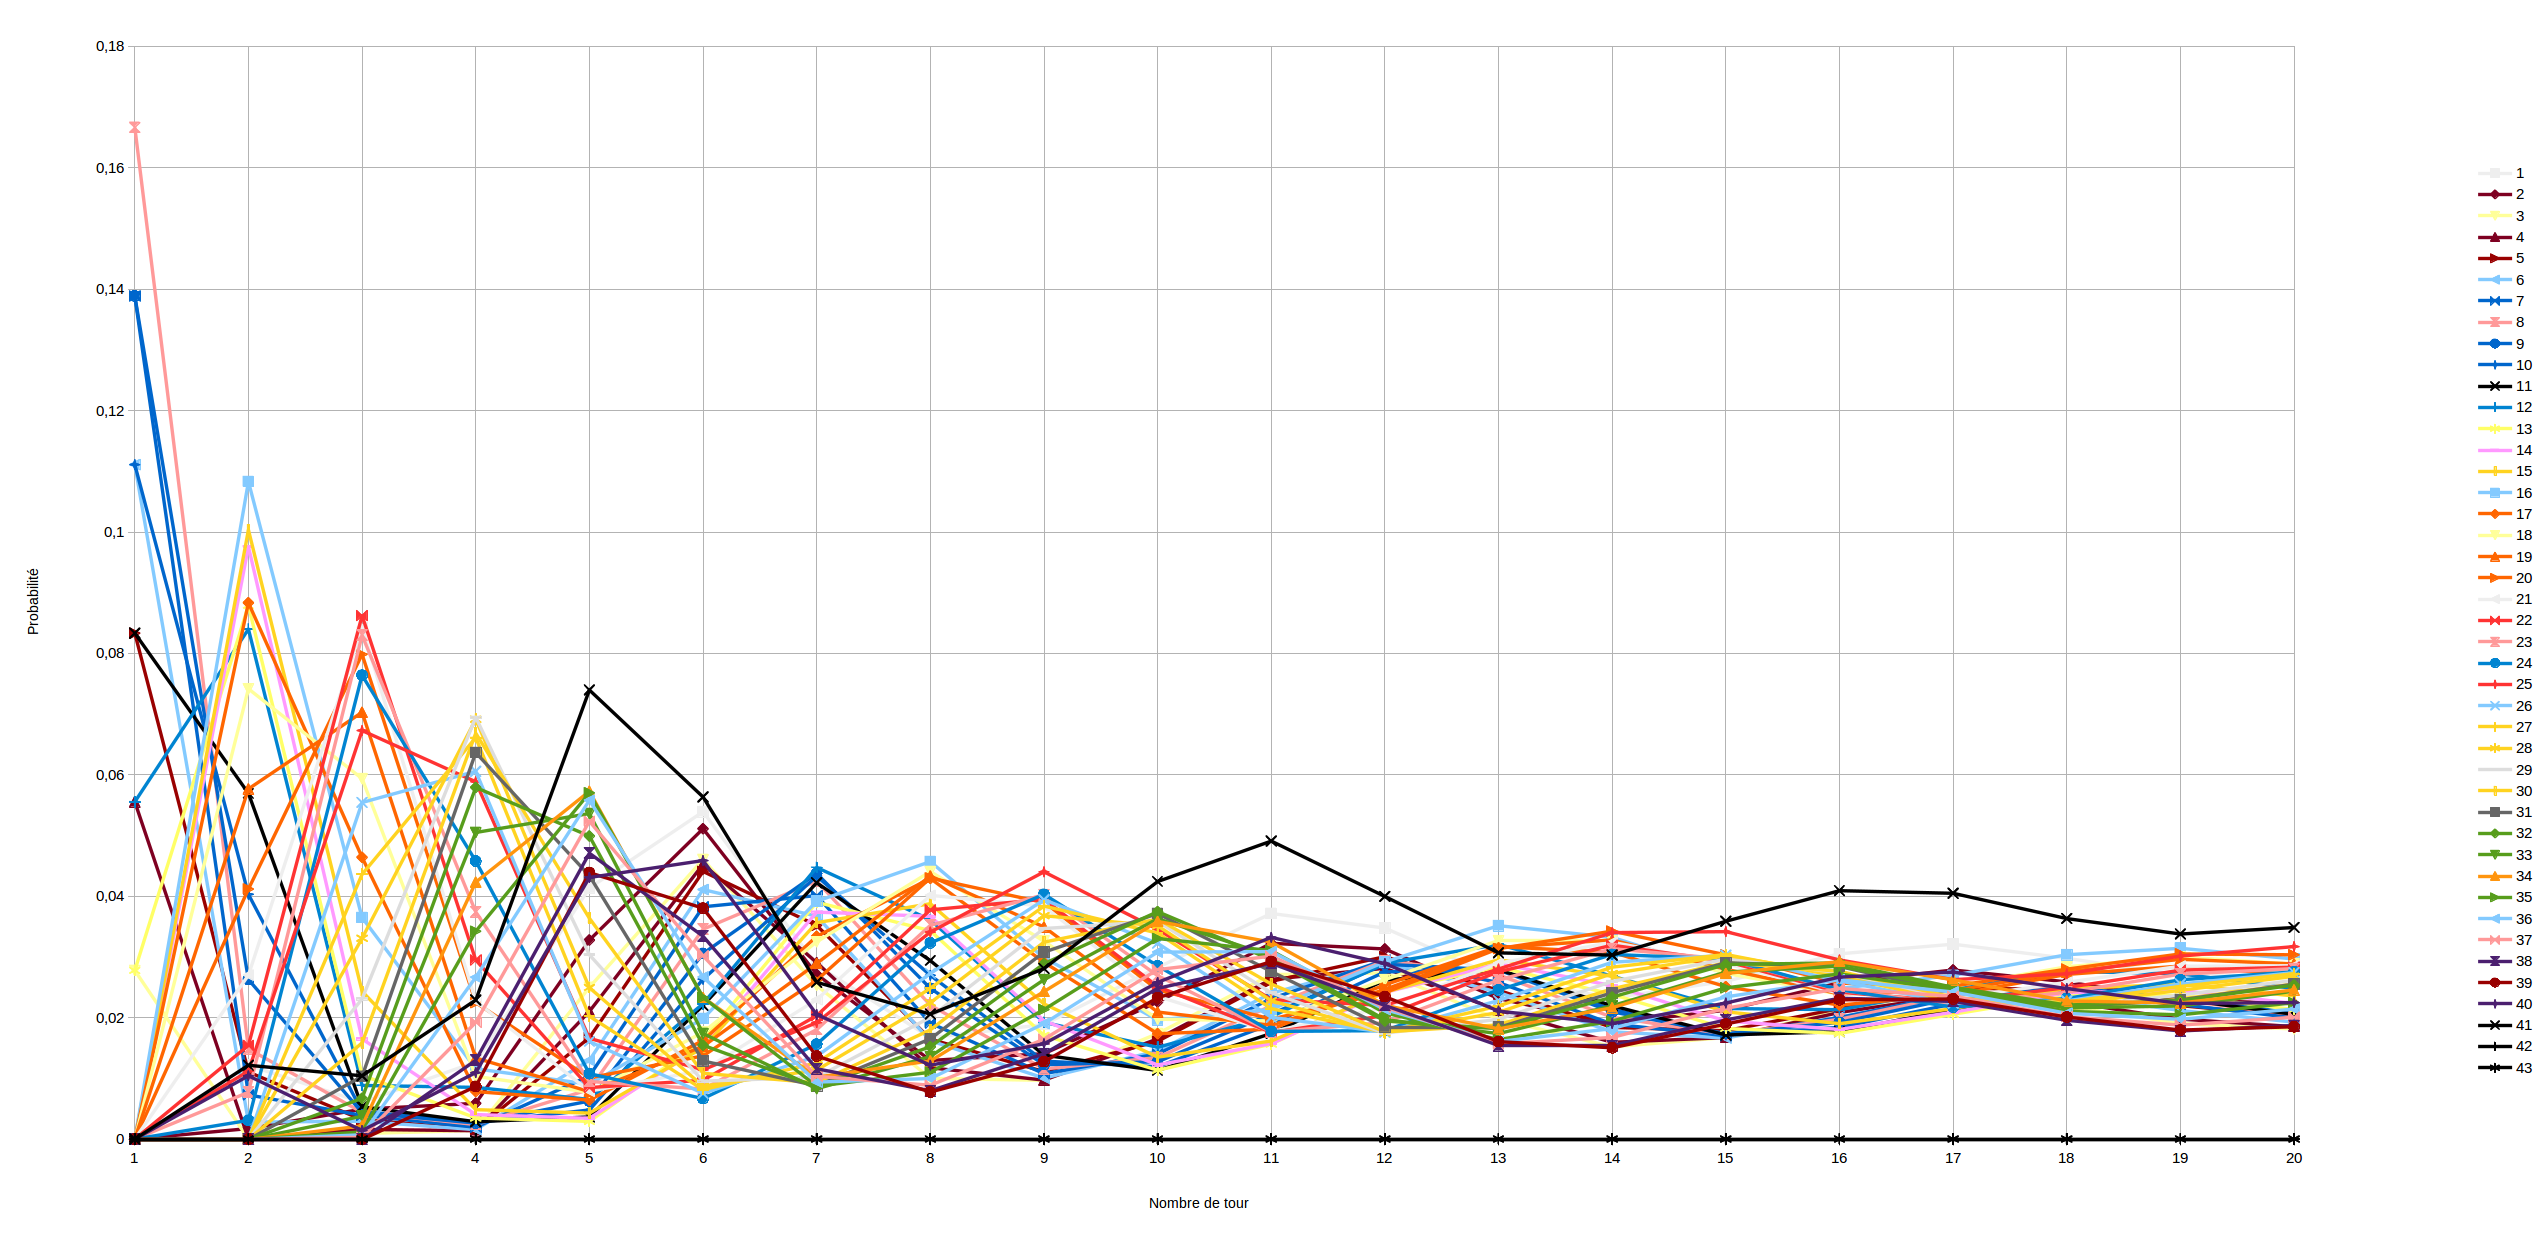
\includegraphics[scale=0.26]{./Images/GraphRepPayeLeq20.png}
	    \caption{\label{graph_result_paye} Répartition des cases entre 1 et 20 tours lorsque le joueur paye directement pour sortir de prison}
	  \end{figure}

	  \begin{figure}[bp!]
	    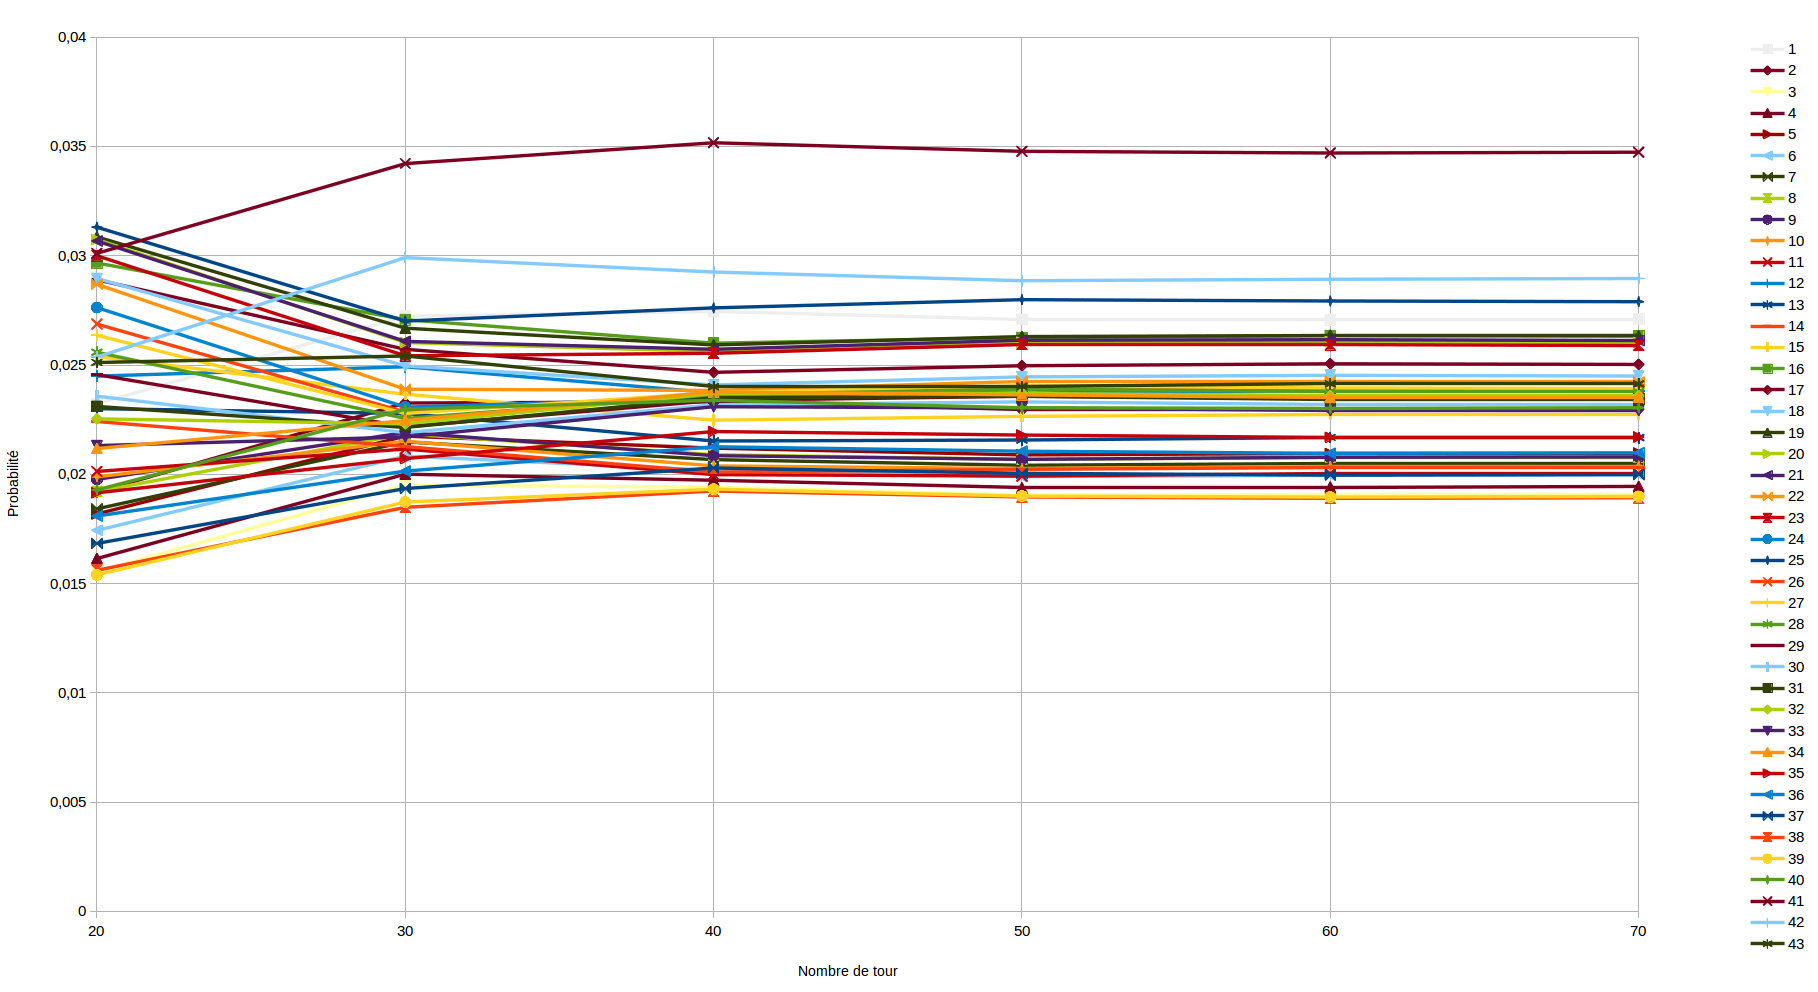
\includegraphics[scale=0.4]{./Images/GraphRepPayePas20-70.png}
	    \caption{\label{graph_all_result_paye_pas} Répartition des cases pour 20, 30, 40, 50, 60 et 70 tours lorsque le joueur ne paye pas pour sortir de prison}
	  \end{figure}

	  \begin{figure}[bp!]
	    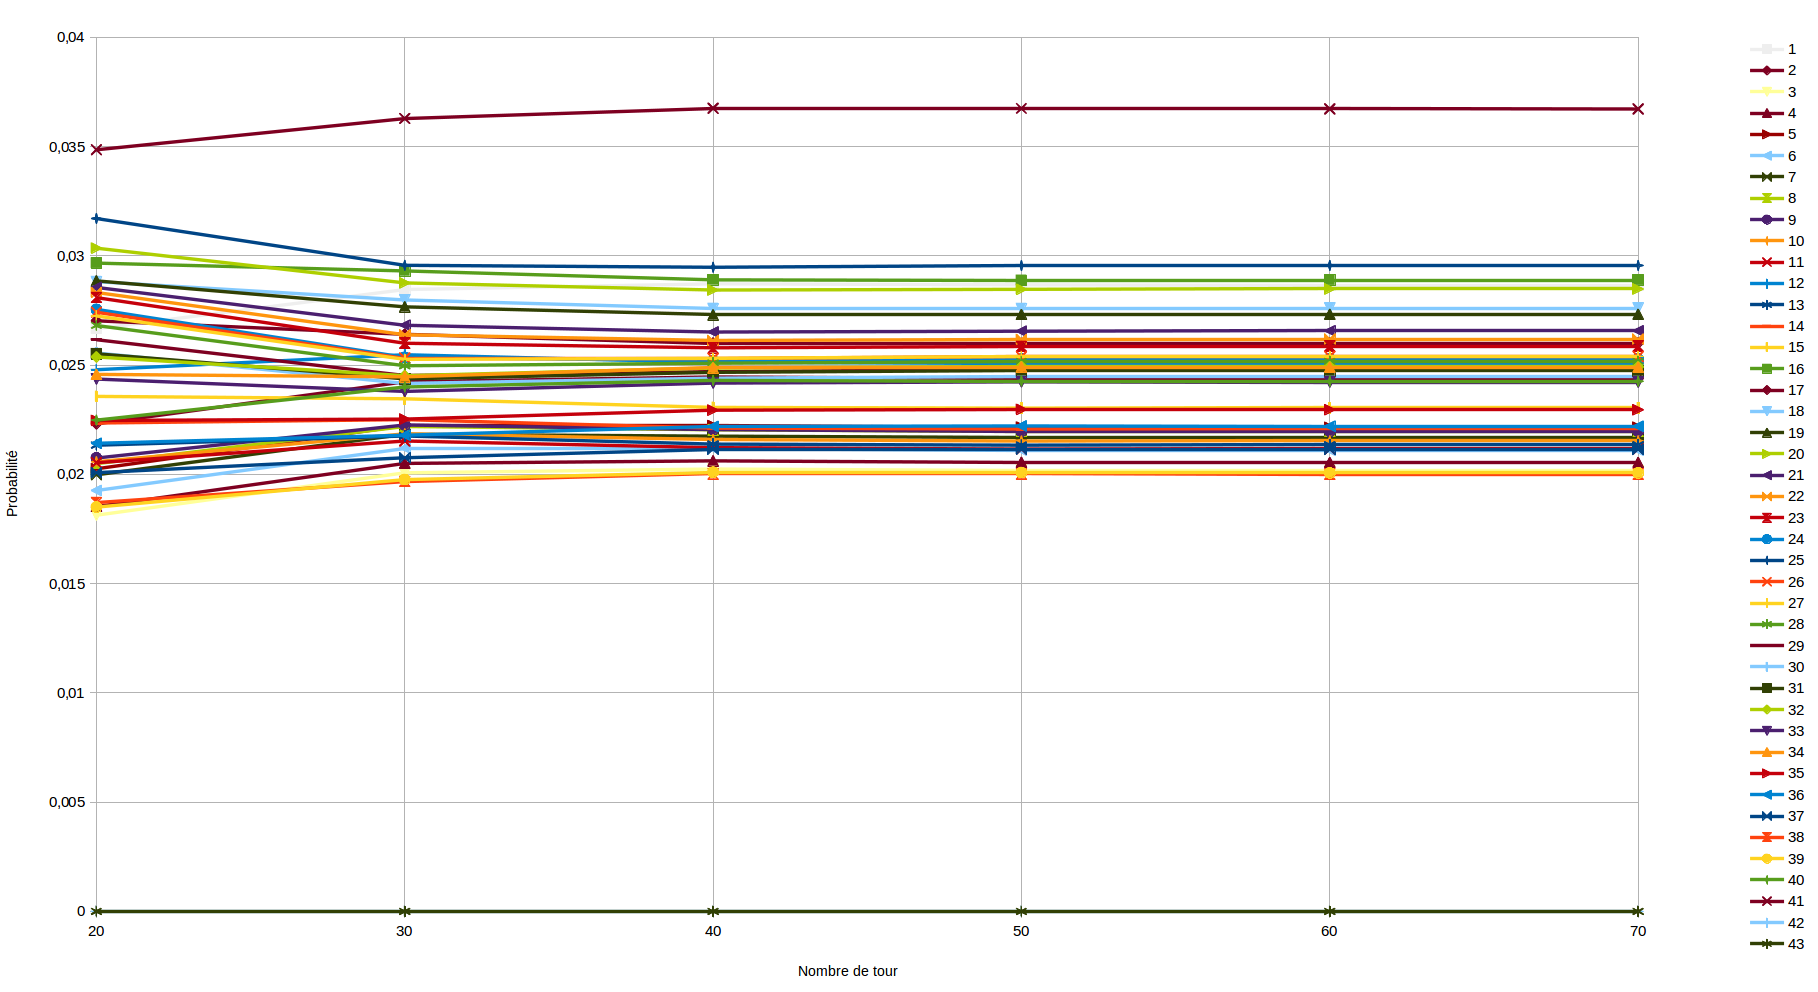
\includegraphics[scale=0.4]{./Images/GraphRepPaye20-70.png}
	    \caption{\label{graph_all_result_paye} Répartition des cases pour 20, 30, 40, 50, 60 et 70 tours lorsque le joueur paye directement pour sortir de prison}
	  \end{figure}
	\end{center}
    \newpage

    \section{Économie des cases}
      \label{annexe:economie}
      \begin{table}[htbp!]
	\centering
	\begin{tabular}{|l|c|c|c||c|c|c|}
	  \hline
	  \multicolumn{1}{|c|}{{\textbf{N}}} & % Numero
	  \multicolumn{1}{p{1.5cm}|}{\centering \textbf{Prix d'achat\\vide}} &
	  \multicolumn{1}{p{1.5cm}|}{\centering \textbf{Revenu terrain vide}} &
	  \multicolumn{1}{p{1.5cm}||}{\centering \textbf{Ratio revenu/prix\\vide}} &
	  \multicolumn{1}{p{1.5cm}|}{\centering \textbf{Prix d'achat\\hotel}} &
	  \multicolumn{1}{p{1.5cm}|}{\centering \textbf{Revenu terrain hotel}} &
	  \multicolumn{1}{p{1.5cm}|}{\centering \textbf{Ratio revenu/prix\\hotel}} \\ \hline %
	  \cellcolor[HTML]{FFFFFF} 1 & - & - & - & - & - & - \\ \hline
	  \cellcolor[HTML]{A0522D} 2 & 600000 \$ & 20000 \$ & 0.033 & 3100000 \$ & 2500000 \$ & 0.806 \\ \hline
	  \cellcolor[HTML]{EEEED1} 3   & - & - & - & - & - & - \\ \hline
	  \cellcolor[HTML]{A0522D} 4 & 600000 \$ & 40000 \$ & 0.067 & 3100000 \$ & 4500000 \$ & 1.452 \\ \hline
	  \cellcolor[HTML]{8B1A1A} \textcolor{white}{5}   & - & - & - & - & - & - \\ \hline
	  \cellcolor[HTML]{E6E6FA} 6 & 2000000 \$ & 250000 \$ & \textbf{0.125} & - & - & - \\ \hline
	  \cellcolor[HTML]{1E90FF} 7 & 1000000 \$ & 60000 \$ & 0.06 & 3500000 \$ & 5500000 \$ & 1.571 \\ \hline
	  \cellcolor[HTML]{FFC1C1} 8   & - & - & - & - & - & - \\ \hline
	  \cellcolor[HTML]{1E90FF} 9 & 1000000 \$ & 60000 \$ & 0.06 & 3500000 \$ & 5500000 \$ & 1.571 \\ \hline
	  \cellcolor[HTML]{1E90FF} 10 & 1200000 \$ & 80000 \$ & 0.067 & 3700000 \$ & 6000000 \$ & \textbf{1.622} \\ \hline
	  \cellcolor[HTML]{000000} \textcolor{white}{11}  & - & - & - & - & - & - \\ \hline
	  \cellcolor[HTML]{FF69B4} 12 & 1400000 \$ & 100000 \$ & 0.071 & 6400000 \$ & 7500000 \$ & 1.172 \\ \hline
	  \cellcolor[HTML]{FFFFF0} 13 & - & - & - & - & - & - \\ \hline
	  \cellcolor[HTML]{FF69B4} 14 & 1400000 \$ & 100000 \$ & 0.071 & 6400000 \$ & 7500000 \$ & 1.172 \\ \hline
	  \cellcolor[HTML]{FF69B4} 15 & 1600000 \$ & 120000 \$ & 0.075 & 6600000 \$ & 9000000 \$ & 1.364 \\ \hline
	  \cellcolor[HTML]{E6E6FA} 16 & 2000000 \$ & 250000 \$ & \textbf{0.125} & - & - & - \\ \hline
	  \cellcolor[HTML]{FF8C00} 17 & 1800000 \$ & 140000 \$ & 0.078 & 6800000 \$ & 9500000 \$ & 1.397 \\ \hline
	  \cellcolor[HTML]{EEEED1} 18  & - & - & - & - & - & - \\ \hline
	  \cellcolor[HTML]{FF8C00} 19 & 1800000 \$ & 140000 \$ & 0.078 & 6800000 \$ & 9500000 \$ & 1.397 \\ \hline
	  \cellcolor[HTML]{FF8C00} 20 & 2000000 \$ & 160000 \$ & 0.08 & 7000000 \$ & 10000000 \$ & 1.429 \\ \hline
	  \cellcolor[HTML]{FFFFFF} 21  & - & - & - & - & - & - \\ \hline
	  \cellcolor[HTML]{FF4500} 22 & 2200000 \$ & 180000 \$ & 0.082 & 9700000 \$ & 10500000 \$ & 1.082 \\ \hline
	  \cellcolor[HTML]{FFC1C1} 23  & - & - & - & - & - & - \\ \hline
	  \cellcolor[HTML]{FF4500} 24 & 2200000 \$ & 180000 \$ & 0.082 & 9700000 \$ & 10500000 \$ & 1.082 \\ \hline
	  \cellcolor[HTML]{FF4500} 25 & 2400000 \$ & 200000 \$ & 0.083 & 9900000 \$ & 11000000 \$ & 1.111 \\ \hline
	  \cellcolor[HTML]{E6E6FA} 26 & 2000000 \$ & 250000 \$ & \textbf{0.125} & - & - & - \\ \hline
	  \cellcolor[HTML]{FFD700} 27 & 2600000 \$ & 220000 \$ & 0.085 & 10100000 \$ & 11500000 \$ & 1.139 \\ \hline
	  \cellcolor[HTML]{FFD700} 28 & 2600000 \$ & 220000 \$ & 0.085 & 10100000 \$ & 11500000 \$ & 1.139 \\ \hline
	  \cellcolor[HTML]{FFFFF0} 29 & - & - & - & - & - & - \\ \hline
	  \cellcolor[HTML]{FFD700} 30 & 2800000 \$ & 240000 \$ & 0.086 & 10300000 \$ & 12000000 \$ & 1.165 \\ \hline
	  \cellcolor[HTML]{BEBEBE} 31  & - & - & - & - & - & - \\ \hline
	  \cellcolor[HTML]{2E8B57} 32 & 3000000 \$ & 260000 \$ & 0.087 & 13000000 \$ & 12750000 \$ & 0.981 \\ \hline
	  \cellcolor[HTML]{2E8B57} 33 & 3000000 \$ & 260000 \$ & 0.087 & 13000000 \$ & 12750000 \$ & 0.981 \\ \hline
	  \cellcolor[HTML]{EEEED1} 34 & - & - & - & - & - & - \\ \hline
	  \cellcolor[HTML]{2E8B57} 35 & 3200000 \$ & 280000 \$ & 0.087 & 13200000 \$ & 14000000 \$ & 1.061 \\ \hline
	  \cellcolor[HTML]{E6E6FA} 36 & 2000000 \$ & 250000 \$ & \textbf{0.125} & - & - & - \\ \hline
	  \cellcolor[HTML]{FFC1C1} 37  & - & - & - & - & - & - \\ \hline
	  \cellcolor[HTML]{483D8B} \textcolor{white}{38} & 3500000 \$ & 350000 \$ & 0.1 & 13500000 \$ & 15000000 \$ & 1.111 \\ \hline
	  \cellcolor[HTML]{8B1A1A} 39  & 1000000 \$ & - & - & 1000000 \$ & - & - \\ \hline
	  \cellcolor[HTML]{483D8B} \textcolor{white}{40} & 4000000 \$ & 500000 \$ & \textbf{0.125} & 14000000 \$ & 20000000 \$ & 1.429 \\ \hline
	\end{tabular}

	\caption{Revenu, prix et ratio de ces deux valeurs pour un joueur qui paye pour sortir de prison}
	\label{table:rentabilite_paye}
      \end{table}

      \begin{table}[h]
	\centering
	\begin{tabular}{|l|c|c|c||c|c|c|}
	  \hline
	  \multicolumn{1}{|c|}{{\textbf{N}}} & % Numero
	  \multicolumn{1}{p{1.5cm}|}{\centering \textbf{Prix d'achat\\vide}} &
	  \multicolumn{1}{p{1.5cm}|}{\centering \textbf{Revenu terrain vide}} &
	  \multicolumn{1}{p{1.5cm}||}{\centering \textbf{Ratio revenu/prix\\vide}} &
	  \multicolumn{1}{p{1.5cm}|}{\centering \textbf{Prix d'achat\\hotel}} &
	  \multicolumn{1}{p{1.5cm}|}{\centering \textbf{Revenu terrain hotel}} &
	  \multicolumn{1}{p{1.5cm}|}{\centering \textbf{Ratio revenu/prix\\hotel}} \\ \hline %
	  \cellcolor[HTML]{FFFFFF} 1 & - & - & - & - & - & - \\ \hline
	  \cellcolor[HTML]{A0522D} 2 & 600000 \$ & 20000 \$ & 0.033 & 3100000 \$ & 2500000 \$ & 0.806 \\ \hline
	  \cellcolor[HTML]{EEEED1} 3   & - & - & - & - & - & - \\ \hline
	  \cellcolor[HTML]{A0522D} 4 & 600000 \$ & 40000 \$ & 0.067 & 3100000 \$ & 4500000 \$ & 1.452 \\ \hline
	  \cellcolor[HTML]{8B1A1A} \textcolor{white}{5}   & 2000000 \$ & - & - & - & - & - \\ \hline
	  \cellcolor[HTML]{E6E6FA} 6 & 2000000 \$ & 250000 \$ & 0.125 & - & - & - \\ \hline
	  \cellcolor[HTML]{1E90FF} 7 & 1000000 \$ & 60000 \$ & 0.06 & 3500000 \$ & 5500000 \$ & 1.571 \\ \hline
	  \cellcolor[HTML]{FFC1C1} 8   & - & - & - & - & - & - \\ \hline
	  \cellcolor[HTML]{1E90FF} 9 & 1000000 \$ & 60000 \$ & 0.06 & 3500000 \$ & 5500000 \$ & 1.571 \\ \hline
	  \cellcolor[HTML]{1E90FF} 10 & 1200000 \$ & 80000 \$ & 0.067 & 3700000 \$ & 6000000 \$ & 1.622 \\ \hline
	  \cellcolor[HTML]{000000} \textcolor{white}{11}  & - & - & - & - & - & - \\ \hline
	  \cellcolor[HTML]{FF69B4} 12 & 1400000 \$ & 100000 \$ & 0.071 & 6400000 \$ & 7500000 \$ & 1.172 \\ \hline
	  \cellcolor[HTML]{FFFFF0} 13 & 1500000 \$ & - & - & - & - & - \\ \hline
	  \cellcolor[HTML]{FF69B4} 14 & 1400000 \$ & 100000 \$ & 0.071 & 6400000 \$ & 7500000 \$ & 1.172 \\ \hline
	  \cellcolor[HTML]{FF69B4} 15 & 1600000 \$ & 120000 \$ & 0.075 & 6600000 \$ & 9000000 \$ & 1.364 \\ \hline
	  \cellcolor[HTML]{E6E6FA} 16 & 2000000 \$ & 250000 \$ & 0.125 & - & - & - \\ \hline
	  \cellcolor[HTML]{FF8C00} 17 & 1800000 \$ & 140000 \$ & 0.078 & 6800000 \$ & 9500000 \$ & 1.397 \\ \hline
	  \cellcolor[HTML]{EEEED1} 18  & - & - & - & - & - & - \\ \hline
	  \cellcolor[HTML]{FF8C00} 19 & 1800000 \$ & 140000 \$ & 0.078 & 6800000 \$ & 9500000 \$ & 1.397 \\ \hline
	  \cellcolor[HTML]{FF8C00} 20 & 2000000 \$ & 160000 \$ & 0.08 & 7000000 \$ & 10000000 \$ & 1.429 \\ \hline
	  \cellcolor[HTML]{FFFFFF} 21  & - & - & - & - & - & - \\ \hline
	  \cellcolor[HTML]{FF4500} 22 & 2200000 \$ & 180000 \$ & 0.082 & 9700000 \$ & 10500000 \$ & 1.082 \\ \hline
	  \cellcolor[HTML]{FFC1C1} 23  & - & - & - & - & - & - \\ \hline
	  \cellcolor[HTML]{FF4500} 24 & 2200000 \$ & 180000 \$ & 0.082 & 9700000 \$ & 10500000 \$ & 1.082 \\ \hline
	  \cellcolor[HTML]{FF4500} 25 & 2400000 \$ & 200000 \$ & 0.083 & 9900000 \$ & 11000000 \$ & 1.111 \\ \hline
	  \cellcolor[HTML]{E6E6FA} 26 & 2000000 \$ & 250000 \$ & 0.125 & - & - & - \\ \hline
	  \cellcolor[HTML]{FFD700} 27 & 2600000 \$ & 220000 \$ & 0.085 & 10100000 \$ & 11500000 \$ & 1.139 \\ \hline
	  \cellcolor[HTML]{FFD700} 28 & 2600000 \$ & 220000 \$ & 0.085 & 10100000 \$ & 11500000 \$ & 1.139 \\ \hline
	  \cellcolor[HTML]{FFFFF0} 29 & 1500000 \$ & - & - & - & - & - \\ \hline
	  \cellcolor[HTML]{FFD700} 30 & 2800000 \$ & 240000 \$ & 0.086 & 10300000 \$ & 12000000 \$ & 1.165 \\ \hline
	  \cellcolor[HTML]{BEBEBE} 31  & - & - & - & - & - & - \\ \hline
	  \cellcolor[HTML]{2E8B57} 32 & 3000000 \$ & 260000 \$ & 0.087 & 13000000 \$ & 12750000 \$ & 0.981 \\ \hline
	  \cellcolor[HTML]{2E8B57} 33 & 3000000 \$ & 260000 \$ & 0.087 & 13000000 \$ & 12750000 \$ & 0.981 \\ \hline
	  \cellcolor[HTML]{EEEED1} 34 & - & - & - & - & - & - \\ \hline
	  \cellcolor[HTML]{2E8B57} 35 & 3200000 \$ & 280000 \$ & 0.087 & 13200000 \$ & 14000000 \$ & 1.061 \\ \hline
	  \cellcolor[HTML]{E6E6FA} 36 & 2000000 \$ & 250000 \$ & 0.125 & - & - & - \\ \hline
	  \cellcolor[HTML]{FFC1C1} 37  & - & - & - & - & - & - \\ \hline
	  \cellcolor[HTML]{483D8B} \textcolor{white}{38} & 3500000 \$ & 350000 \$ & 0.1 & 13500000 \$ & 15000000 \$ & 1.111 \\ \hline
	  \cellcolor[HTML]{8B1A1A} 39  & 1000000 \$ & - & - & - & - & - \\ \hline
	  \cellcolor[HTML]{483D8B} \textcolor{white}{40} & 4000000 \$ & 500000 \$ & 0.125 & 14000000 \$ & 20000000 \$ & 1.429 \\ \hline
	\end{tabular}
	\caption{Revenu, prix et ratio de ces deux valeurs pour un joueur qui ne paye pas pour sortir de prison}
	\label{table:rentabilite_paye_pas}
      \end{table}
      

\end{document}
